\documentclass[journal]{IEEEtran}

\usepackage{cite}
\usepackage{amsmath}
\usepackage{amssymb}
\usepackage{graphicx}
\usepackage{booktabs}
\usepackage{url}

\graphicspath{{../figures/v2/}{../figures/}}

\interdisplaylinepenalty=2500

\begin{document}

\title{VanniKawachh: A Distributed AI Acoustic Intelligence and Autonomous
Drone Response Network for Women Safety}

\author{Shivansh~Verma,
        Saksham~Sabadra,
        Rudra~Thakur,
        and~Rohan~Untawale%
\thanks{The authors are with the Department of Computer Science and
Engineering, G H Raisoni College of Engineering, Nagpur, India.}%
\thanks{This work was carried out under the guidance of Dr.~Aditya Turankar,
Assistant Professor, Department of Computer Science and Engineering,
G H Raisoni College of Engineering, Nagpur, India.}}

\markboth{Journal of \LaTeX\ Class Files}%
{Verma \MakeLowercase{\textit{et al.}}: VanniKawachh: A Distributed AI Acoustic Intelligence and Autonomous Drone Response Network}

\maketitle

\begin{abstract}
Most crimes against women occur precisely where existing safety technology
fails: dark streets, forest paths, and no-signal parking areas. Prevailing
solutions shift the burden of safety onto the potential victim, who must carry
a device, install an application, keep it charged, and reach for it at the
worst possible moment. VanniKawachh removes that burden. Solar-powered
microphone nodes mounted on poles listen continuously for acoustic distress
events (``Bachao!'', ``Help!'', screams). A two-stage artificial-intelligence
pipeline keeps false alarms low: each node's ESP32-S3 microcontroller screens
every second of audio with a lightweight MFCC-plus-CNN classifier (Stage~1,
under 50~ms per frame), and a Raspberry Pi~5 hub confirms candidate events
with PANNs deep audio analysis fused with motion, ambient-light, and
time-of-day evidence (Stage~2). Confirmed alerts---AES-128 encrypted and
carrying the node's surveyed GPS coordinates---travel over LoRa, requiring no
SIM card or cellular coverage, to a police dashboard, and simultaneously
auto-dispatch a Pixhawk quadcopter that records evidence at the scene and
delivers a first-aid kit. The response chain is protected by a safety
framework comprising telemetry-verified flight-mode delivery, a debounced
severity-ordered failsafe arbiter, and a landing-interlocked mission queue. We
present the system architecture, the cryptographic alert protocol, and the
flight-safety framework, validated by software-in-the-loop acceptance flights
(8/8 checks passed, 0.4~m terminal accuracy), 68 automated unit
verifications, and a complete end-to-end chain rehearsal from sealed alert to
payload release. Her voice is the only safety device she needs.
\end{abstract}

\begin{IEEEkeywords}
Women's safety, acoustic event detection, MFCC, CNN, PANNs, LoRa, AES
encryption, GPS, autonomous quadcopter, Pixhawk.
\end{IEEEkeywords}

\IEEEpeerreviewmaketitle

\section{Introduction}

\IEEEPARstart{P}{ublic}-safety statistics and case studies repeatedly show
that violent crimes against women concentrate in locations with poor
infrastructure coverage: unlit streets, isolated stretches between transit
stops, forest and campus peripheries, and underground or remote parking
areas. These are exactly the locations where the two dominant classes of
safety technology break down. Cellular-network-dependent applications lose
connectivity; camera surveillance requires lighting, power, and a human
observer; and personal devices require the victim to possess, charge, and
physically operate them during an assault.

This last point deserves emphasis, because it is a structural flaw rather
than an engineering one. Nearly every deployed women-safety
solution---smartphone applications, smart wearables, GPS panic
buttons---implements a \emph{victim-carried} trigger. The system works only
if the woman (i)~owns the device, (ii)~is carrying it, (iii)~has kept it
charged, (iv)~has network coverage, and (v)~can reach and operate it during
the seconds in which an attack unfolds. Each condition is individually
plausible and jointly fragile. Reported detection accuracies of such devices
exceed 97\%~\cite{bharathi2025}, yet the accuracy is conditioned on the
device being present and usable---a condition the threat model itself
undermines, since an assailant's first action is often to separate the victim
from her phone.

VanniKawachh (``Vanni''---voice; ``Kawachh''---shield) inverts the
responsibility. The sensing infrastructure is mounted on public poles,
powered by solar energy, and listens continuously; the victim carries
nothing. Her voice---a scream, a cry, the keywords ``help'' or
``bachao''---is the trigger. Detection, verification, alerting, and physical
first response are all performed by fixed and aerial infrastructure.

The contributions of this paper are as follows.
\begin{enumerate}
\item \textbf{An end-to-end architecture} for infrastructure-mounted acoustic
women-safety sensing, spanning solar-powered ESP32-S3 sensing nodes, a
Raspberry Pi~5 verification hub, and an autonomous Pixhawk quadcopter
response layer, in which no component depends on cellular coverage or a
victim-carried device.
\item \textbf{A two-stage acoustic verification pipeline} that pairs a
recall-tuned, sub-50~ms on-node MFCC+CNN screen with a precision-tuned hub
stage combining PANNs~\cite{kong2020} deep audio tagging and a weighted
fusion of PIR motion, ambient light, and time-of-day evidence, including a
defined degraded-mode path when the verification clip cannot be delivered.
\item \textbf{A 25-byte authenticated alert protocol} for LoRa, using
AES-128-CTR confidentiality, truncated HMAC-SHA256 authenticity, per-node key
derivation from a single master key, and monotonic-counter replay
protection---sized to a single LoRa frame and designed around the observation
that a spoofed packet would launch an aircraft.
\item \textbf{A safety-verified autonomous response framework} for the
dispatch drone: telemetry-confirmed flight-mode delivery with layered MAVLink
re-encoding and cross-action emergency fallback; a landing-interlocked serial
mission queue; a debounced, severity-ordered failsafe arbiter; geofence
validation at the network edge; and a payload-delivery phase whose failure
mode is return-to-launch, never loiter. These mechanisms are the subject of
two patent applications in preparation.
\item \textbf{Software-in-the-loop (SITL) validation} of the complete
response chain---8/8 acceptance checks, 0.4~m terminal accuracy, 68 automated
unit verifications, and a full-chain rehearsal from sealed alert packet to
simulated first-aid drop---together with an honest statement of which
measurements remain pending on physical hardware.
\end{enumerate}

The remainder of the paper is organized as follows.
Section~\ref{sec:related} surveys related work and identifies the gap
VanniKawachh addresses. Section~\ref{sec:architecture} presents the
three-tier architecture. Sections~\ref{sec:acoustic}--\ref{sec:safety} detail
the acoustic verification pipeline, the secure alerting protocol, and the
flight-safety framework, respectively. Section~\ref{sec:results} reports
experimental results and explicitly delimits validated claims from pending
measurements. Section~\ref{sec:discussion} discusses privacy, regulatory
context, and limitations. Section~\ref{sec:conclusion} concludes.

\section{Related Work}
\label{sec:related}

Prior work on technology for women's safety and acoustic distress detection
falls into two broad categories: systems the victim must carry, and systems
that detect but do not respond.

\subsection{Victim-Carried Devices and Applications}

Pavithra \emph{et al.}~\cite{pavithra2026} present a discreet smartphone
application with on-device audio recognition and emergency automation; the
design is thoughtful, but the trigger chain still requires the victim's own
charged, network-connected phone. Bharathi \emph{et
al.}~\cite{bharathi2025} describe an IoT wearable combining GPS and
accelerometer sensing, reporting 97.54\% detection accuracy, a 3.2~s
response time, and a 1.92\% false-positive rate---strong figures that
nonetheless apply only while the wearable is worn and charged. Snehith
\emph{et al.}~\cite{snehith2025} and Hadkar \emph{et al.}~\cite{hadkar2024}
present IoT safety devices in which a push-button or wearable initiates
locate-and-alert behavior; both require manual triggering by the victim.
Uganya \emph{et al.}~\cite{uganya2023} describe a button-triggered GSM/GPS
tracker, which is inoperative exactly in the GSM dead zones where risk is
highest. Potturi \emph{et al.}~\cite{potturi2026} automate the SOS trigger
with GSM/GPS geo-location sharing but retain both the carried-device and
cellular-coverage dependencies. Across this category, reported accuracies are
high, but the burden of possession, charge, coverage, and reach remains on
the victim.

\subsection{Detection-Only Acoustic Systems}

A second body of work detects distress sounds without providing location
delivery or physical response. Kim \emph{et al.}~\cite{kim2024} built an
11,921-sample large-scale scream dataset and found a CNN-Transformer to be
the best of five evaluated models; the system is server-scale and terminates
at detection. The same group~\cite{kim2025} later proposed a CNN-Transformer
with a windowing CNN for scream temporal-interval prediction, improving
F-measure by roughly three percentage points and equal-error rate by an
order of magnitude---but the model is compute-heavy and not deployable on
low-power field nodes. Sharma and Jebaseeli~\cite{sharma2025} report a
scream-and-panic detector at 92\% accuracy with under 5\% false positives
and 4--6~s response, bound to the user's device. Srimathi \emph{et
al.}~\cite{srimathi2025} show that scream detection can reduce reaction time
by 40\% and increase intervention rates by 30\%, underscoring the
operational value of acoustic sensing, but their system is single-stage and
offers no field response. Fime \emph{et al.}~\cite{fime2024} achieve 95.51\%
danger-sound accuracy with Noisereduce preprocessing and InceptionV3,
identifying MobileNetV2 as a lighter alternative---again, detection only.
Ciaburro and Puyana-Romero~\cite{ciaburro2026} systematically review
sound-event detection in smart cities and confirm both the maturity of
detection methods and the near-absence of closed-loop response systems in
the literature.

\subsection{The Gap}

Table~\ref{tab:positioning} summarizes the pattern. Victim-carried systems
close the response loop but place the trigger burden on the victim;
detection-only systems remove that burden but stop at a classification
score. To the best of our knowledge, no prior system provides the complete
chain of \emph{infrastructure-mounted sensing} (no victim burden),
\emph{verified low-false-alarm alerting that operates offline} (no cellular
dependency), and \emph{autonomous physical field response} (aid arrives
before ground units). VanniKawachh is designed to fill exactly this gap.

\begin{table*}[!t]
\caption{Positioning of VanniKawachh Against Prior Work}
\label{tab:positioning}
\centering
\begin{tabular}{@{}lccc@{}}
\toprule
Property &
Victim-carried \cite{pavithra2026,bharathi2025,snehith2025,hadkar2024,uganya2023,potturi2026} &
Detection-only \cite{kim2025,sharma2025,srimathi2025,kim2024,fime2024} &
VanniKawachh \\
\midrule
Victim must carry/charge a device & Yes & No & No \\
Works without cellular coverage & Mostly no & N/A (server-side) & Yes (LoRa) \\
Deployable on low-power field nodes & Yes & Mostly no & Yes (two-stage split) \\
False-alarm suppression stage & No & Single-stage & Two-stage + sensor fusion \\
Location delivered to responders & Yes (live GPS) & No & Yes (surveyed registry) \\
Autonomous physical response & No & No & Yes (quadcopter) \\
\bottomrule
\end{tabular}
\end{table*}

\section{System Architecture}
\label{sec:architecture}

VanniKawachh comprises three tiers: per-pole sensing nodes, a per-locality
hub, and a response drone, as shown in Fig.~\ref{fig:architecture}. The
design principle uniting all three is that \emph{a detection claimed is not
a detection confirmed}---every layer independently verifies before it acts,
whether the object of verification is a sound, a network packet, or a
flight-mode command.

\begin{figure*}[!t]
\centering
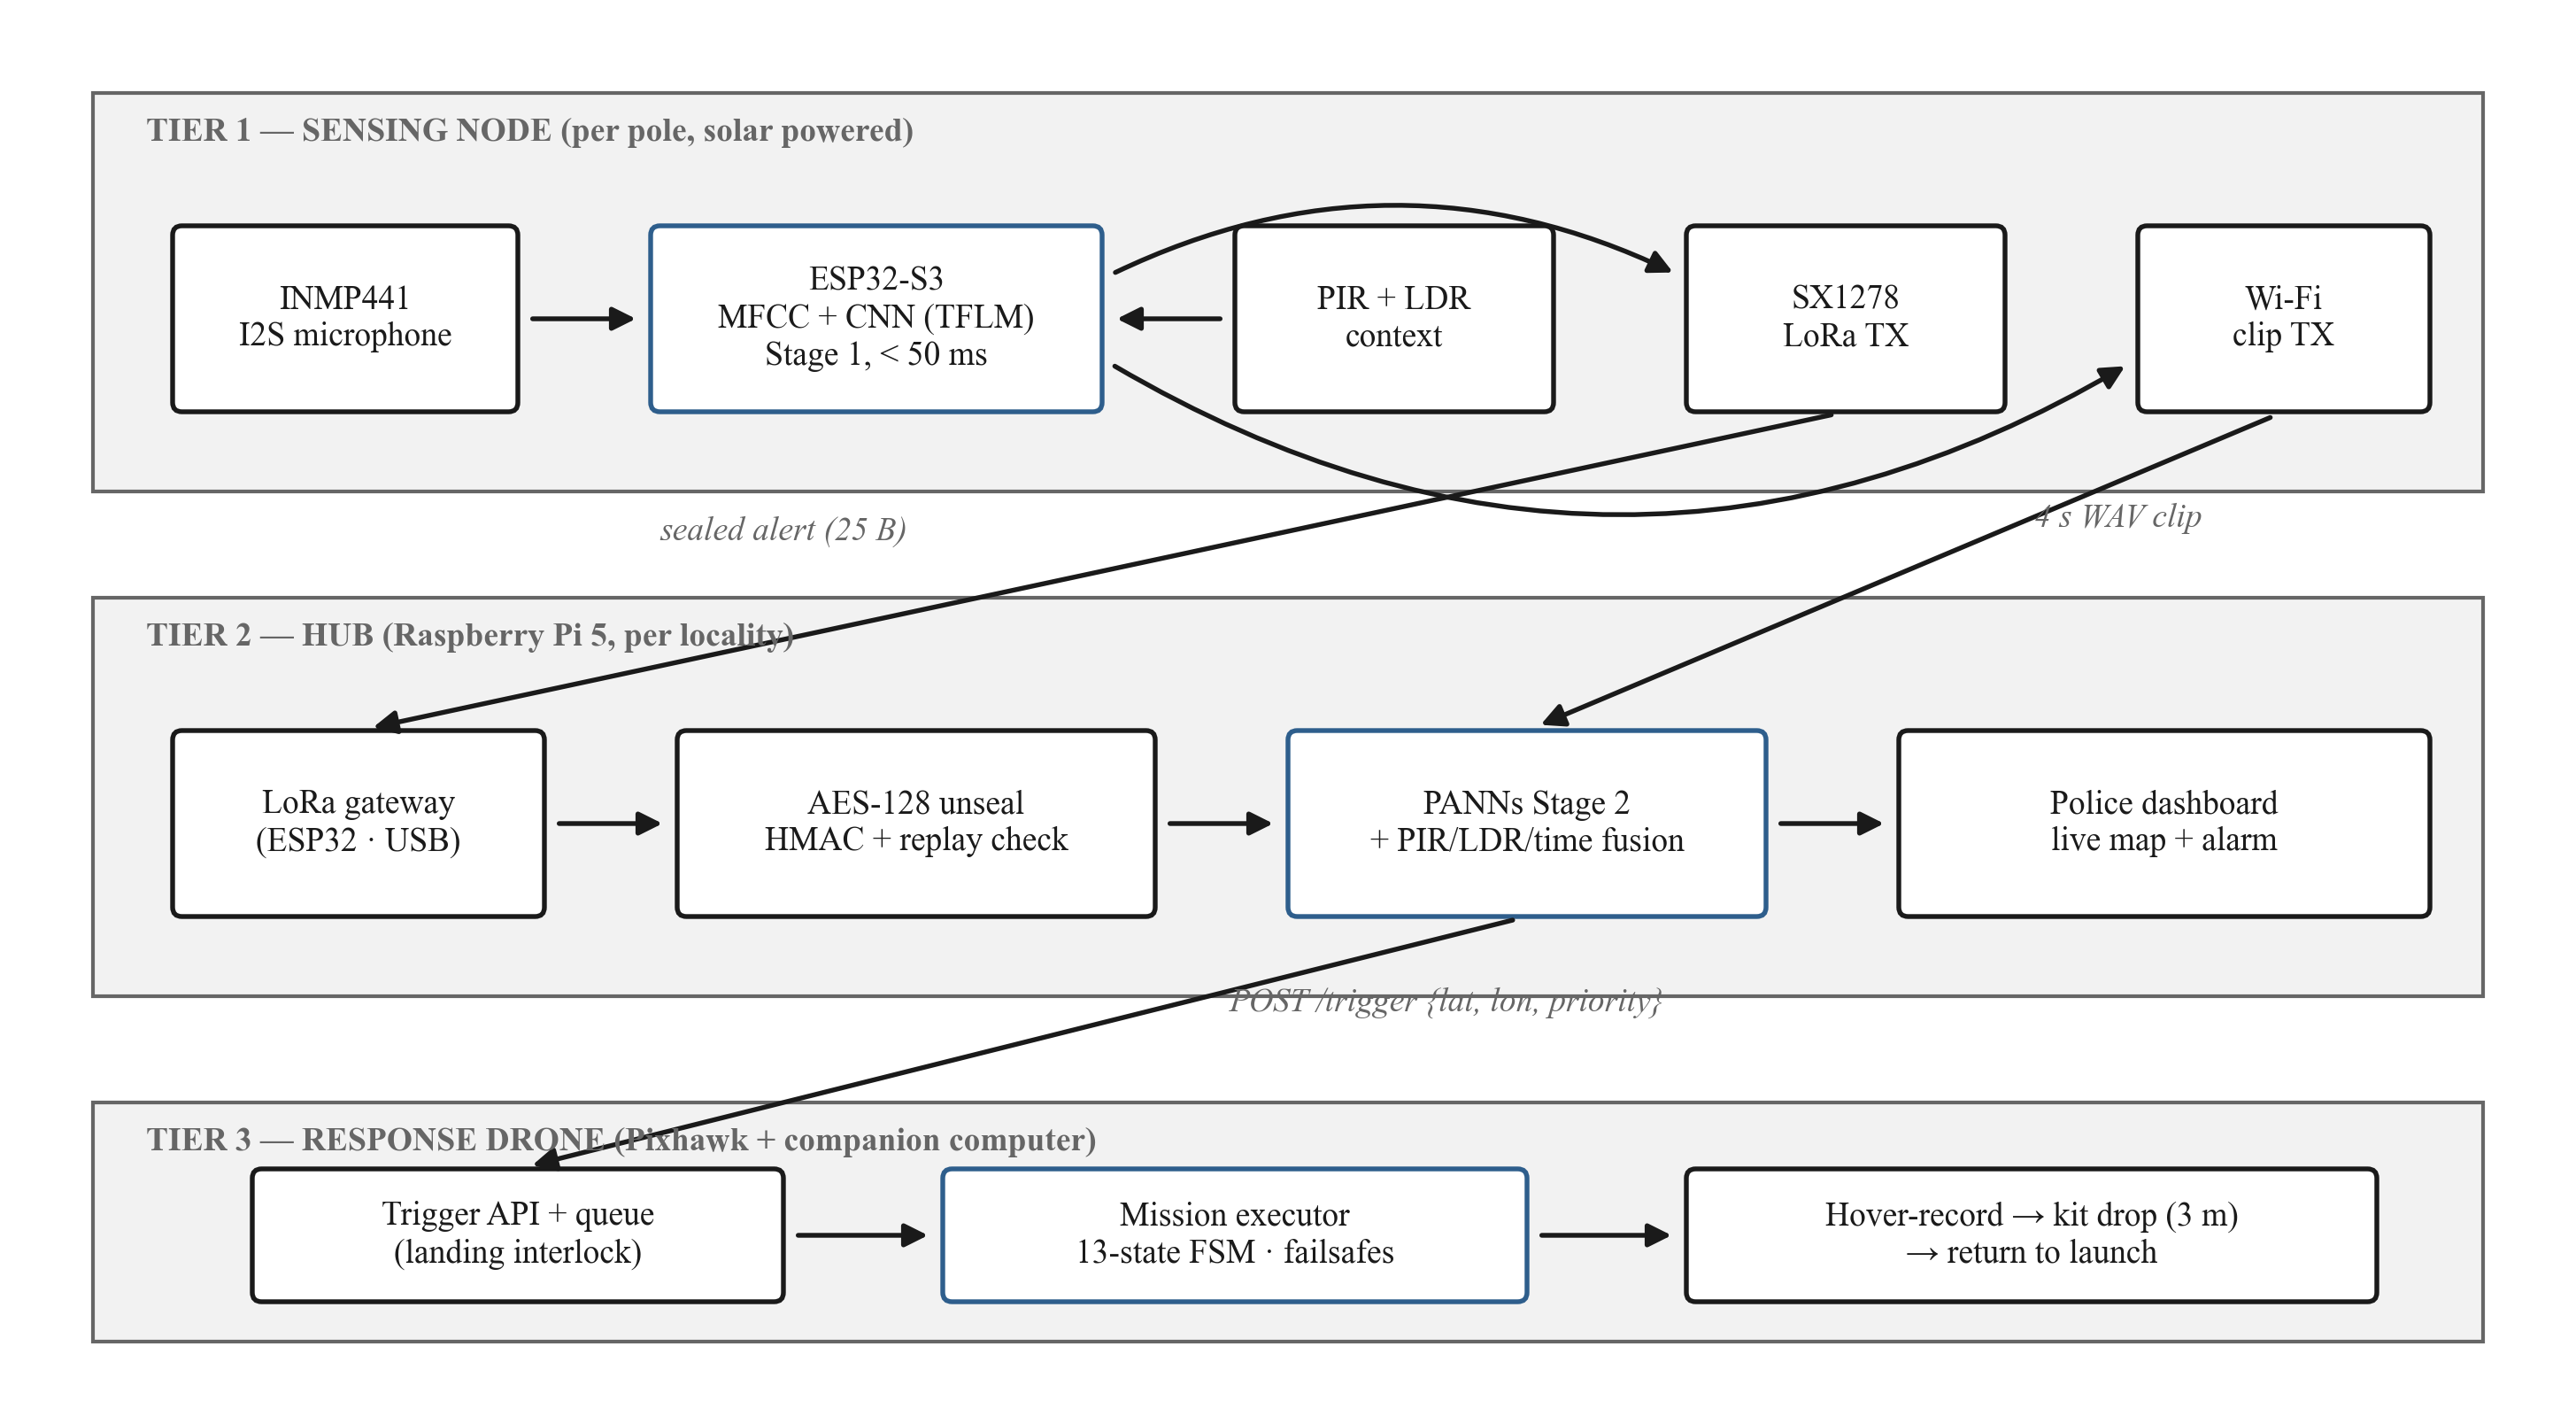
\includegraphics[width=\textwidth]{fig1_architecture.png}
\caption{System architecture of the VanniKawachh network: solar-powered
sensing nodes (Tier~1), the Raspberry Pi~5 verification hub (Tier~2), and
the autonomous response drone (Tier~3), linked by LoRa alerts and
ESP-NOW/WiFi clips.}
\label{fig:architecture}
\end{figure*}

\subsection{Tier 1: Sensing Node}

Each node is a weatherproof, solar-powered unit (ESP32-S3 microcontroller;
INMP441 I2S MEMS microphone sampling 16~kHz mono; HC-SR501 PIR motion
sensor; LDR ambient-light sensor; SX1278 LoRa transceiver at 433~MHz; 18650
Li-ion cell with TP4056 charging from a 5~V solar panel). The ESP32-S3
continuously frames incoming audio, extracts MFCC features, and runs a
lightweight convolutional classifier under TensorFlow Lite for
Microcontrollers~\cite{david2021}, budgeted at under 50~ms per frame. Audio
that does not resemble distress is discarded on-device---nothing is stored
and nothing is transmitted. On a Stage-1 hit, the node (i)~transmits a
sealed 25-byte alert over LoRa (Section~\ref{sec:alerting}) and (ii)~uploads
a 4~s verification clip over ESP-NOW/WiFi to the hub. Nodes carry no GPS:
each pole is surveyed once at installation, and position is resolved at the
hub from a \texttt{node\_id} $\rightarrow$ (lat, lon) registry. A node
therefore has no live position fix to spoof, jam, or drain.

\subsection{Tier 2: Hub}

The hub is a Raspberry Pi~5 serving one locality. A gateway ESP32 with an
SX1278 receives LoRa frames and bridges them to the Pi over USB serial; the
gateway performs no cryptography or parsing, so all security-relevant logic
remains on the Pi, where it can be updated without reflashing field
hardware. The hub authenticates and decrypts each alert, checks the replay
counter, looks up the node registry, waits a bounded time for the
verification clip, runs Stage-2 audio analysis (PANNs~\cite{kong2020}),
fuses the result with the alert's PIR/light flags and the time of day
(Section~\ref{sec:acoustic}), and---only above configured
thresholds---dispatches the drone by an HTTP POST to the flight stack's
trigger interface while raising the incident on a police-facing dashboard
with a live map and alarm.

\subsection{Tier 3: Response Drone}

The response layer is a Pixhawk 2.4.8 quadcopter (F450 class) with an
onboard companion computer running the flight stack: a FastAPI trigger
interface with a bounded priority queue, a 13-state mission executor (IDLE,
CONNECTING, WAITING\_GPS, ARMING, TAKEOFF, ENROUTE, HOVERING, DELIVERING,
RTL, LANDED, COMPLETED, ABORTED, FAILED), a 1~Hz failsafe arbiter, and
obstacle keep-out routing. The drone flies to the node's surveyed
coordinates in GUIDED mode over MAVLink~\cite{ardupilot}, records camera
evidence during hover, descends to release a first-aid kit, and returns to
launch. The complete safety machinery is described in
Section~\ref{sec:safety}.

\subsection{Methodology Flow}

Fig.~\ref{fig:methodology} traces one incident through the system, from the
acoustic event through both verification stages to the parallel dashboard
and drone-dispatch paths.

\begin{figure}[!t]
\centering
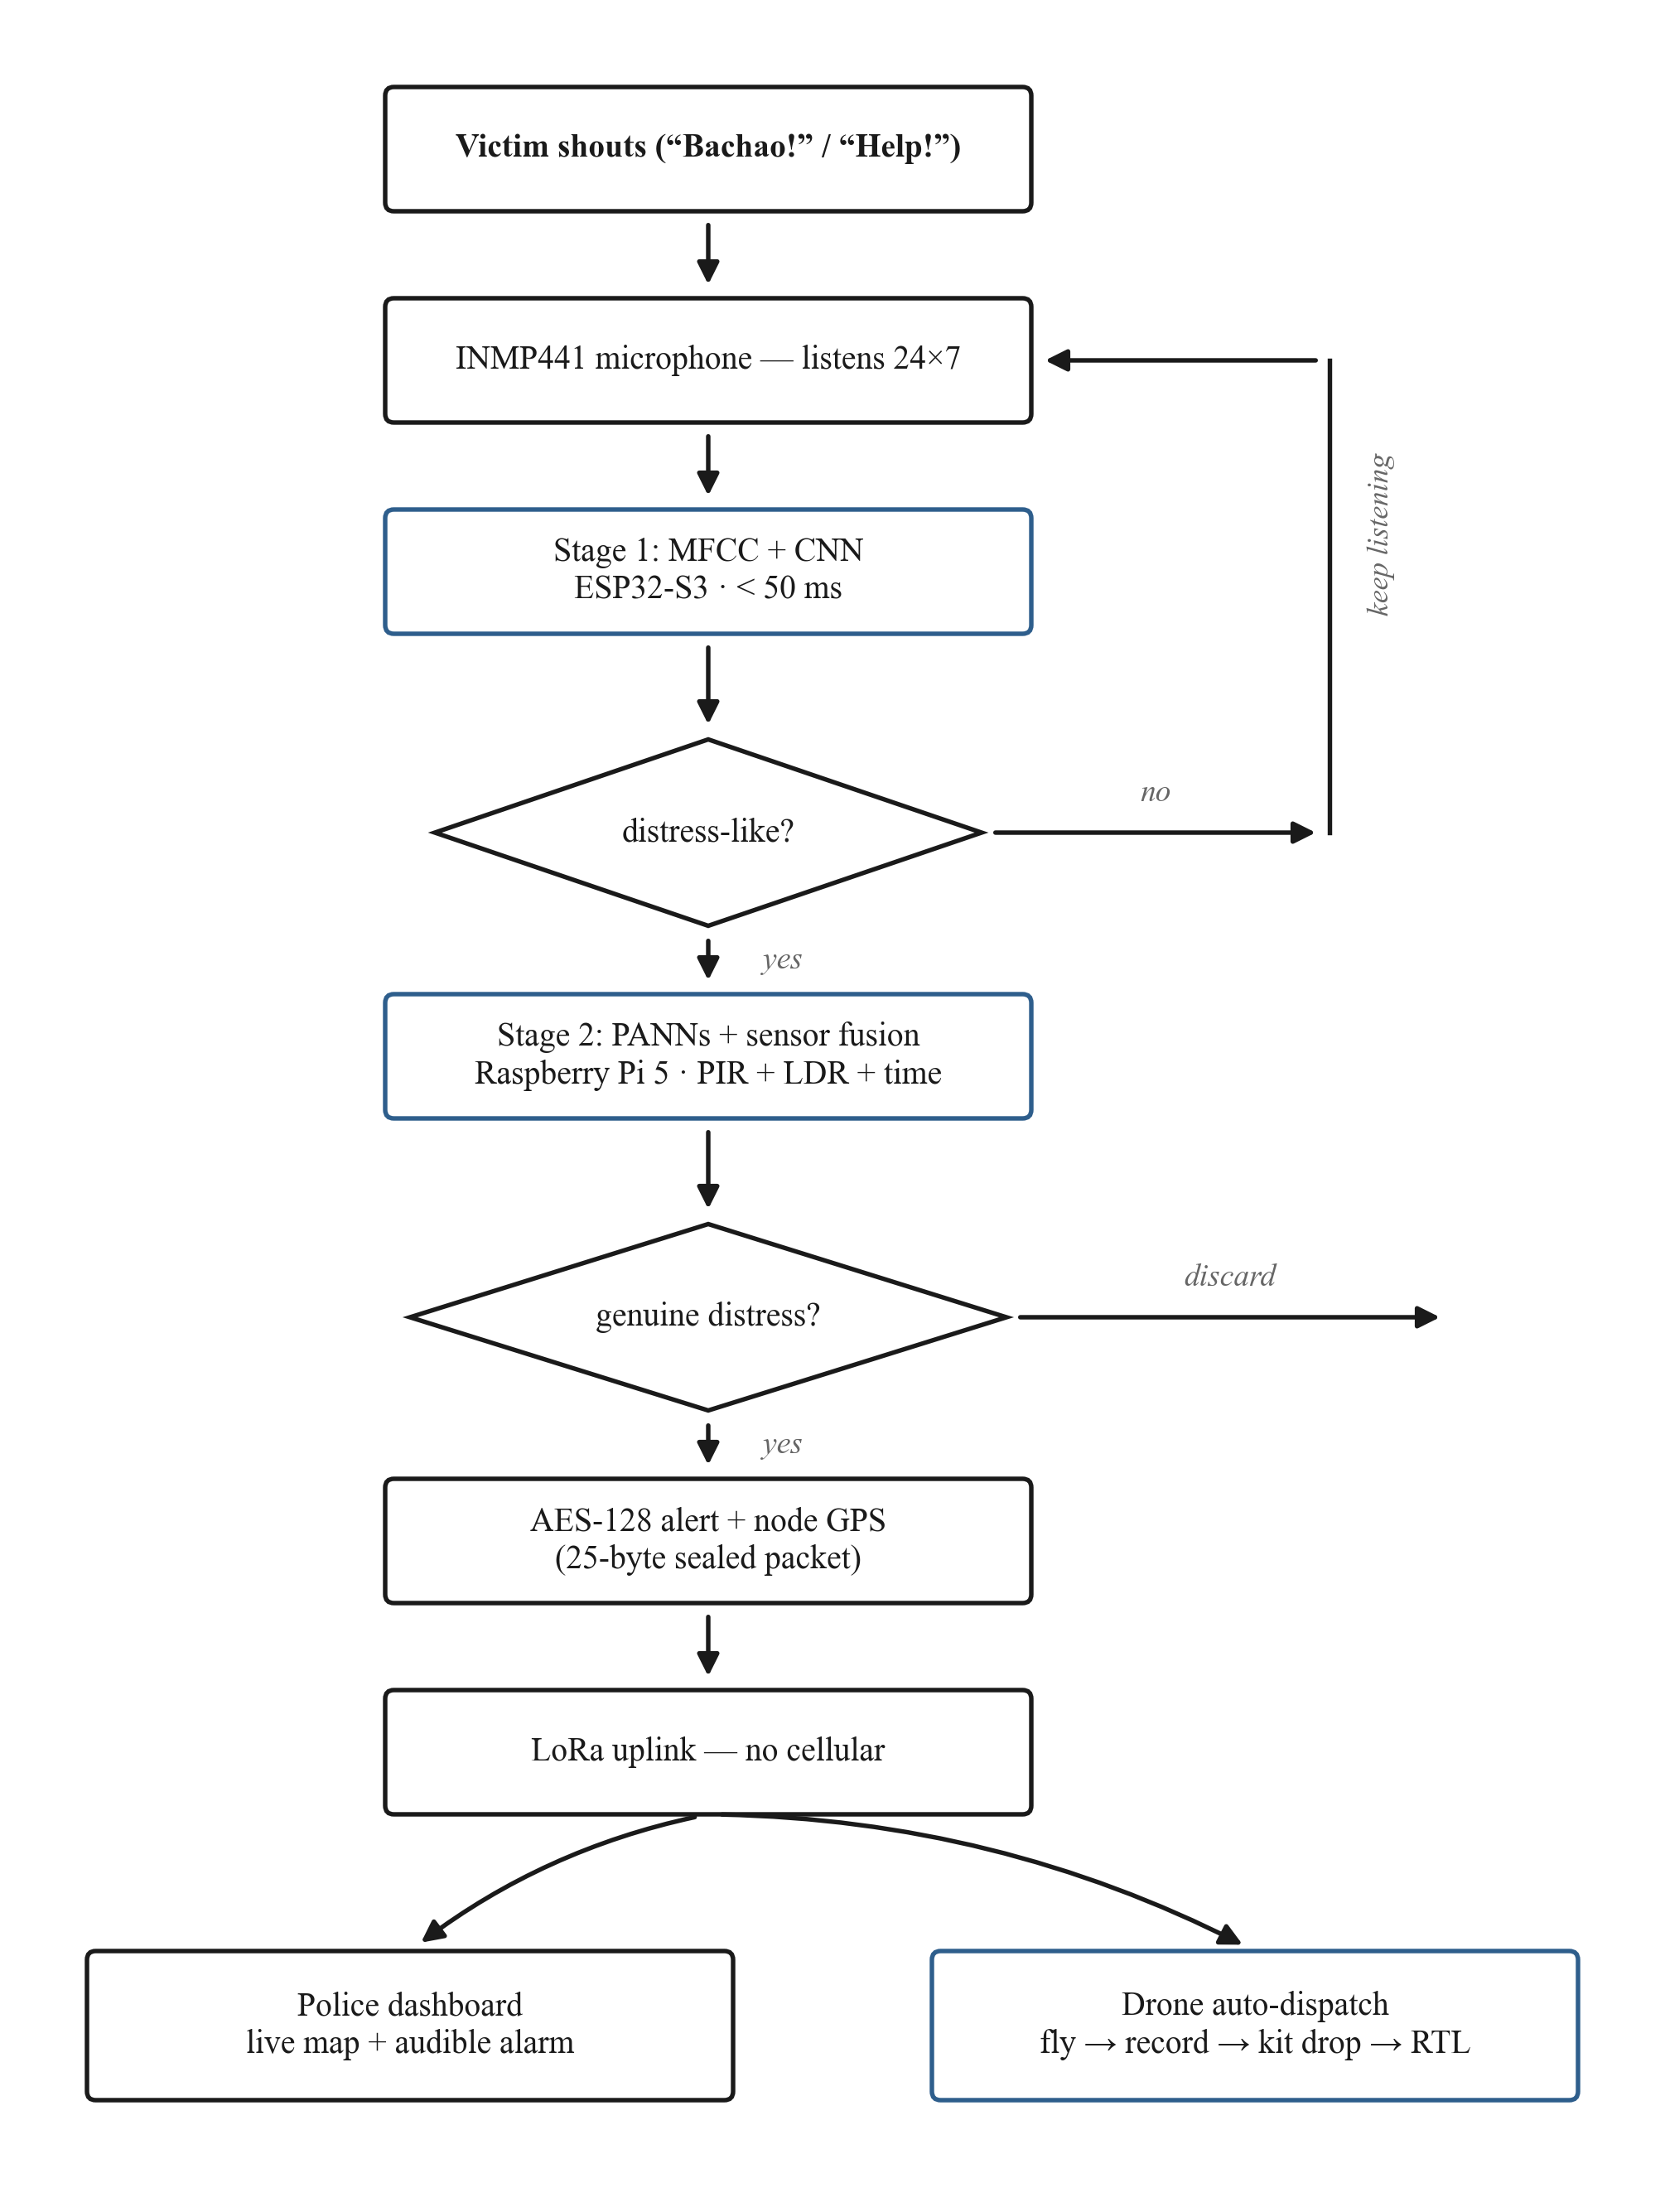
\includegraphics[width=\columnwidth]{fig2_methodology.png}
\caption{VanniKawachh methodology flow from acoustic event to autonomous
response: Stage-1 on-node screening, Stage-2 hub verification and fusion,
sealed LoRa alerting, and the parallel police-dashboard and drone-dispatch
paths ending in the first-aid kit drop and return to launch.}
\label{fig:methodology}
\end{figure}

\section{Two-Stage Acoustic Verification}
\label{sec:acoustic}

The acoustic pipeline is split across the node and the hub because the two
requirements---never miss a real event, and never launch on a false
one---pull in opposite directions and are best served by different operating
points on different hardware.

\subsection{Stage 1: Recall-Tuned On-Node Screening}

The node computes MFCCs over short frames of the 16~kHz microphone stream
and classifies them with a compact CNN of the \texttt{micro\_speech} class
under TensorFlow Lite for Microcontrollers~\cite{david2021}, targeting
scream, cry, and the keywords ``help'' and ``bachao''. The Stage-1 signal
chain, shown in Fig.~\ref{fig:pipeline}, is the standard speech front end.
Each frame is first pre-emphasized to flatten the spectral tilt of voiced
audio,
\begin{equation}
\label{eq:preemphasis}
y[n] = x[n] - 0.97\,x[n-1],
\end{equation}
and multiplied by a Hamming window to bound spectral leakage,
\begin{equation}
\label{eq:hamming}
w[n] = 0.54 - 0.46\cos\!\left(\frac{2\pi n}{N-1}\right),
\quad 0 \leq n \leq N-1 .
\end{equation}
The magnitude spectrum of each windowed frame is pooled by a bank of $M$
triangular filters spaced uniformly on the mel scale,
\begin{equation}
\label{eq:mel}
m = 2595\,\log_{10}\!\left(1 + \frac{f}{700}\right),
\end{equation}
which mimics the ear's compressive frequency resolution---the resolution at
which screams and shouted keywords are most separable from traffic and wind.
The log filterbank energies
\begin{equation}
\label{eq:fbank}
e_j = \log \sum_{k} |X(k)|^{2}\,H_j(k), \quad j = 1, \ldots, M,
\end{equation}
are decorrelated by a DCT-II to yield the cepstral coefficients
\begin{equation}
\label{eq:dct}
c_i = \sum_{j=1}^{M} e_j \cos\!\left[\frac{i\left(j -
\tfrac{1}{2}\right)\pi}{M}\right], \quad i = 1, \ldots, 13,
\end{equation}
of which the first 13 form the per-frame feature vector.

\begin{figure}[!t]
\centering
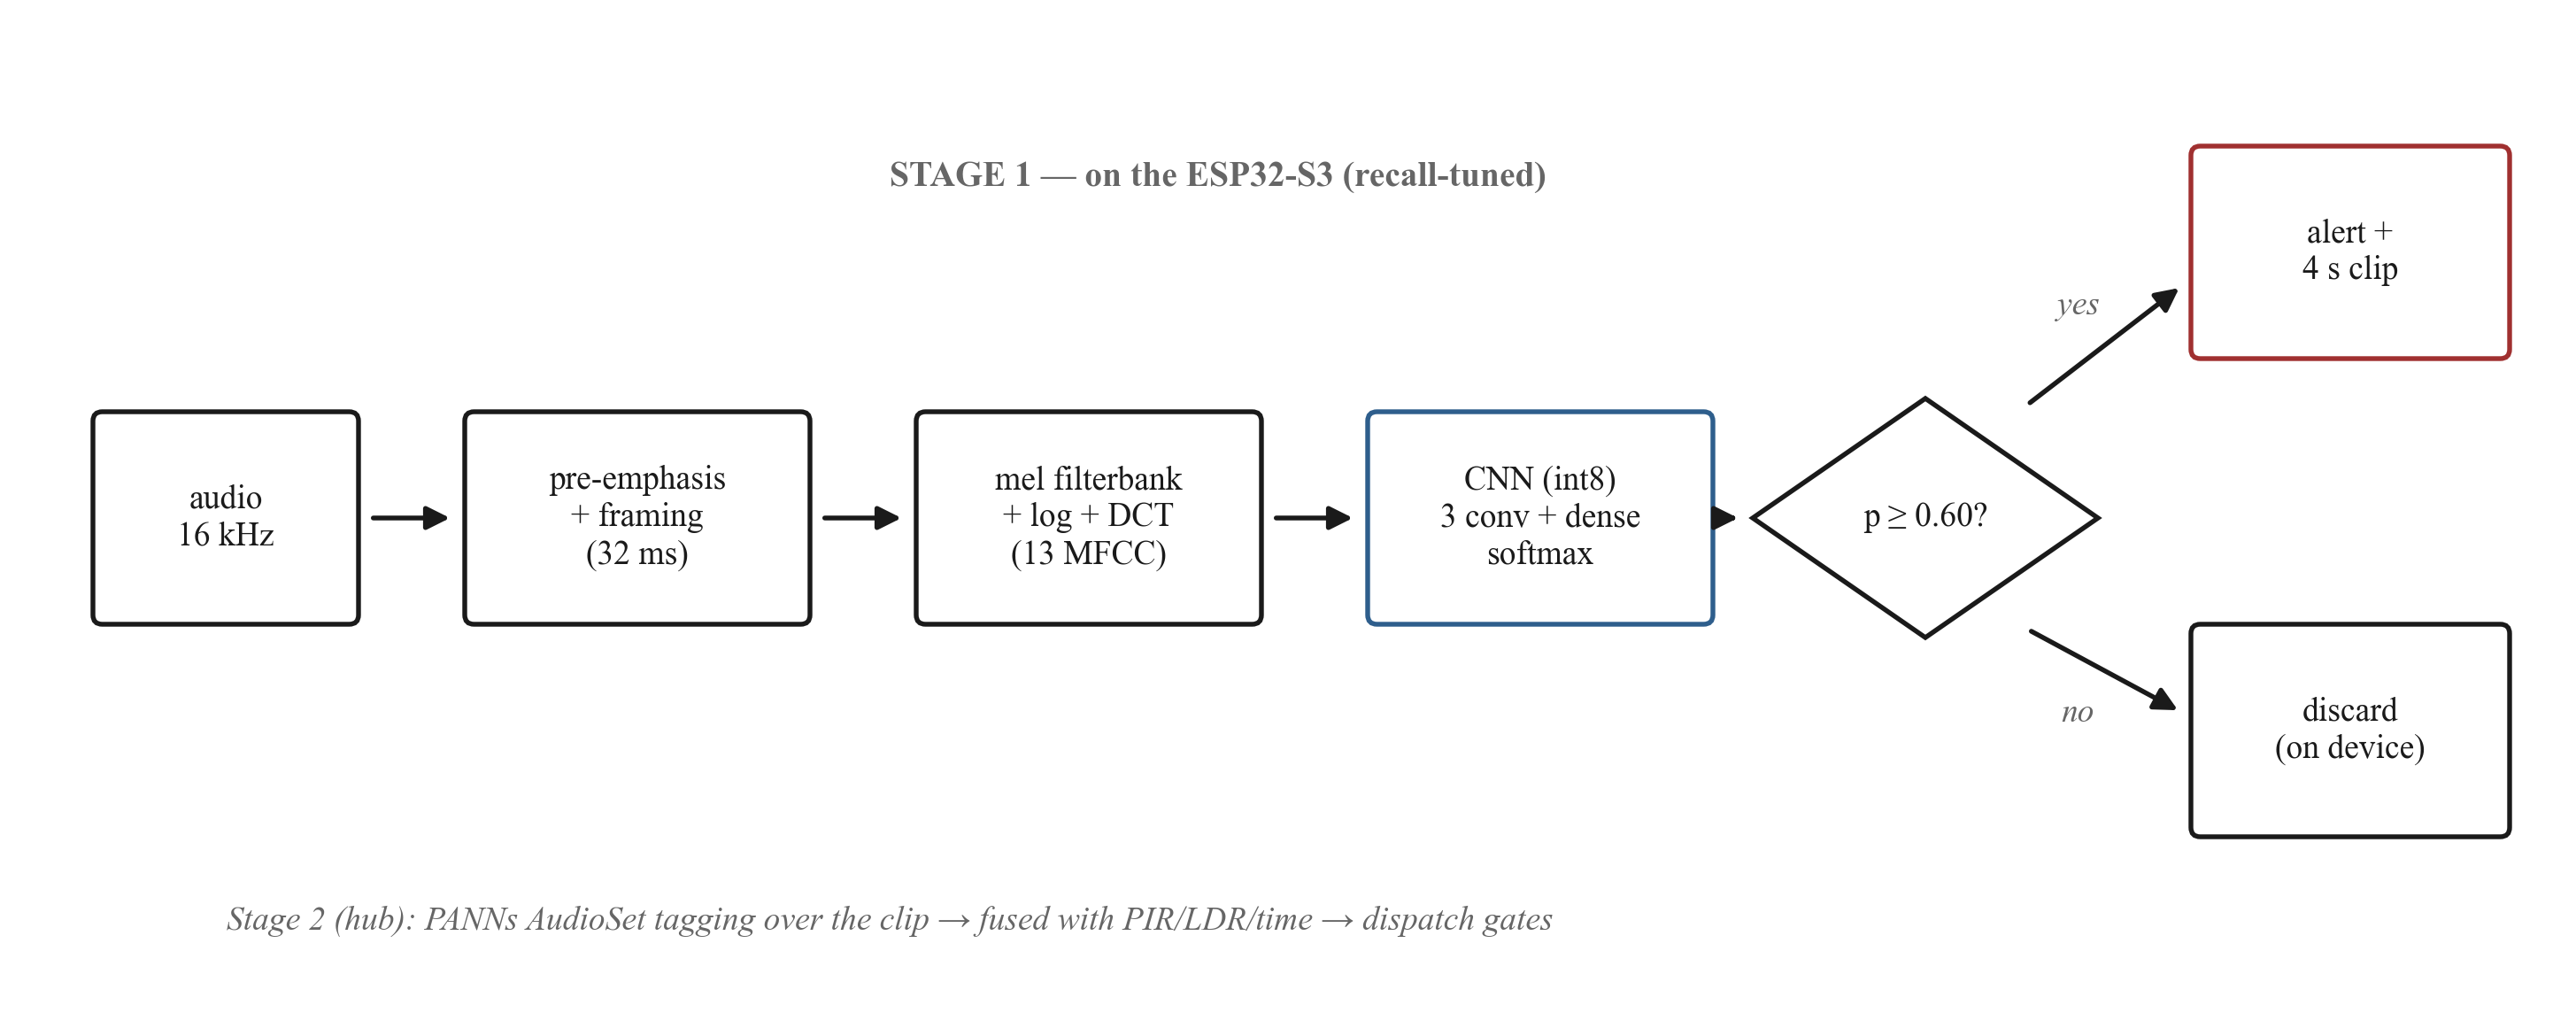
\includegraphics[width=\columnwidth]{fig3_pipeline.png}
\caption{Stage-1 signal chain on the sensing node: pre-emphasis, windowing,
mel filterbank, DCT-II cepstrum, and the quantized CNN classifier, all
within the sub-50~ms frame budget.}
\label{fig:pipeline}
\end{figure}

The MFCC frames feed a compact convolutional classifier whose output layer
is a softmax over the distress vocabulary,
\begin{equation}
\label{eq:softmax}
p_i = \frac{\exp(z_i)}{\sum_{j} \exp(z_j)},
\end{equation}
trained by minimizing the cross-entropy loss against one-hot labels $y$,
\begin{equation}
\label{eq:crossentropy}
\mathcal{L} = -\sum_{i} y_i \log p_i .
\end{equation}
For deployment, the trained weights and activations are converted to 8-bit
integers by post-training quantization,
\begin{equation}
\label{eq:quantization}
x_q = \operatorname{round}(x/s) + z,
\end{equation}
with per-tensor scale $s$ and zero-point $z$; int8 execution is what lets
the model fit within the ESP32-S3's memory and the TFLM interpreter's kernel
set. The stage is deliberately \emph{recall-tuned}: its purpose is to not
miss distress, and its false positives are cheap because Stage~2 filters
them at the hub. The latency budget is under 50~ms per frame so that the
node keeps pace with real time on the ESP32-S3's resources. In the current
prototype, the deployed Stage-1 classifier is a calibrated energy/band
heuristic standing in for the trained TFLM model; model training on
scream/keyword corpora is scheduled as Phase~1 of the build plan
(Section~\ref{sec:pending}).

\subsection{Stage 2: Precision-Tuned Hub Verification}

The hub scores the 4~s verification clip with PANNs~\cite{kong2020}, a
family of large-scale pretrained audio neural networks trained on AudioSet.
The distress score is the summed clipwise probability over the
distress-relevant AudioSet classes (screaming, shouting, yelling, crying,
wailing, groaning, whimpering), yielding a value in $[0, 1]$. CNN14 is the
default checkpoint, with CNN10 or a MobileNet variant as substitutes if
inference on the Pi~5 proves too slow. The verifier also implements an
energy-heuristic fallback backend (loudness, spectral centroid, and envelope
burstiness; specified exactly in
\eqref{eq:rms}--\eqref{eq:heuristic} of Section~\ref{sec:rehearsal}) so that
the full pipeline remains executable and testable on machines without
PyTorch; this fallback is explicitly not a claim of detection accuracy and
is labeled as such wherever results are reported.

\subsection{Evidence Fusion}

A night-time scream in a dark spot with motion nearby warrants a different
response from a daytime shout on a busy road. The hub therefore fuses the
Stage-2 audio score with environmental evidence carried in the alert packet,
as shown in Fig.~\ref{fig:fusion}. With $a$ the Stage-2 audio score, $c$ the
Stage-1 confidence, $p \in \{0,1\}$ the PIR motion flag, $L \in [0,255]$ the
LDR light level, and $h$ the local hour of day, the fused severity is
\begin{equation}
\label{eq:fusion}
S = 0.60\,a + 0.15\,c + 0.10\,p + 0.08\,d + 0.07\,n,
\end{equation}
where darkness $d = 1 - L/255$ and the night indicator $n \in \{0,1\}$
equals 1 if $h \geq 20$ or $h < 6$ (20:00--06:00), else 0; $S$ is clamped to
$[0, 1]$. Audio evidence dominates (weight 0.60), while each contextual
factor nudges severity upward. Dispatch requires both gates of
\eqref{eq:dispatch} to pass:
\begin{equation}
\label{eq:dispatch}
\text{dispatch} \;\Leftrightarrow\; (a \geq \tau_v) \wedge (S \geq \tau_d),
\quad \tau_v = 0.50, \ \tau_d = 0.60,
\end{equation}
and mission priority is set to \emph{high} when $S \geq 0.75$, or when
$a \geq 0.6$ with motion confirmed ($p = 1$); otherwise \emph{normal}.
Alerts below threshold are logged for audit but do not launch the drone;
this gating is pinned by unit tests. The weights are prototype values to be
tuned against Phase-1 bench data.

\begin{figure}[!t]
\centering
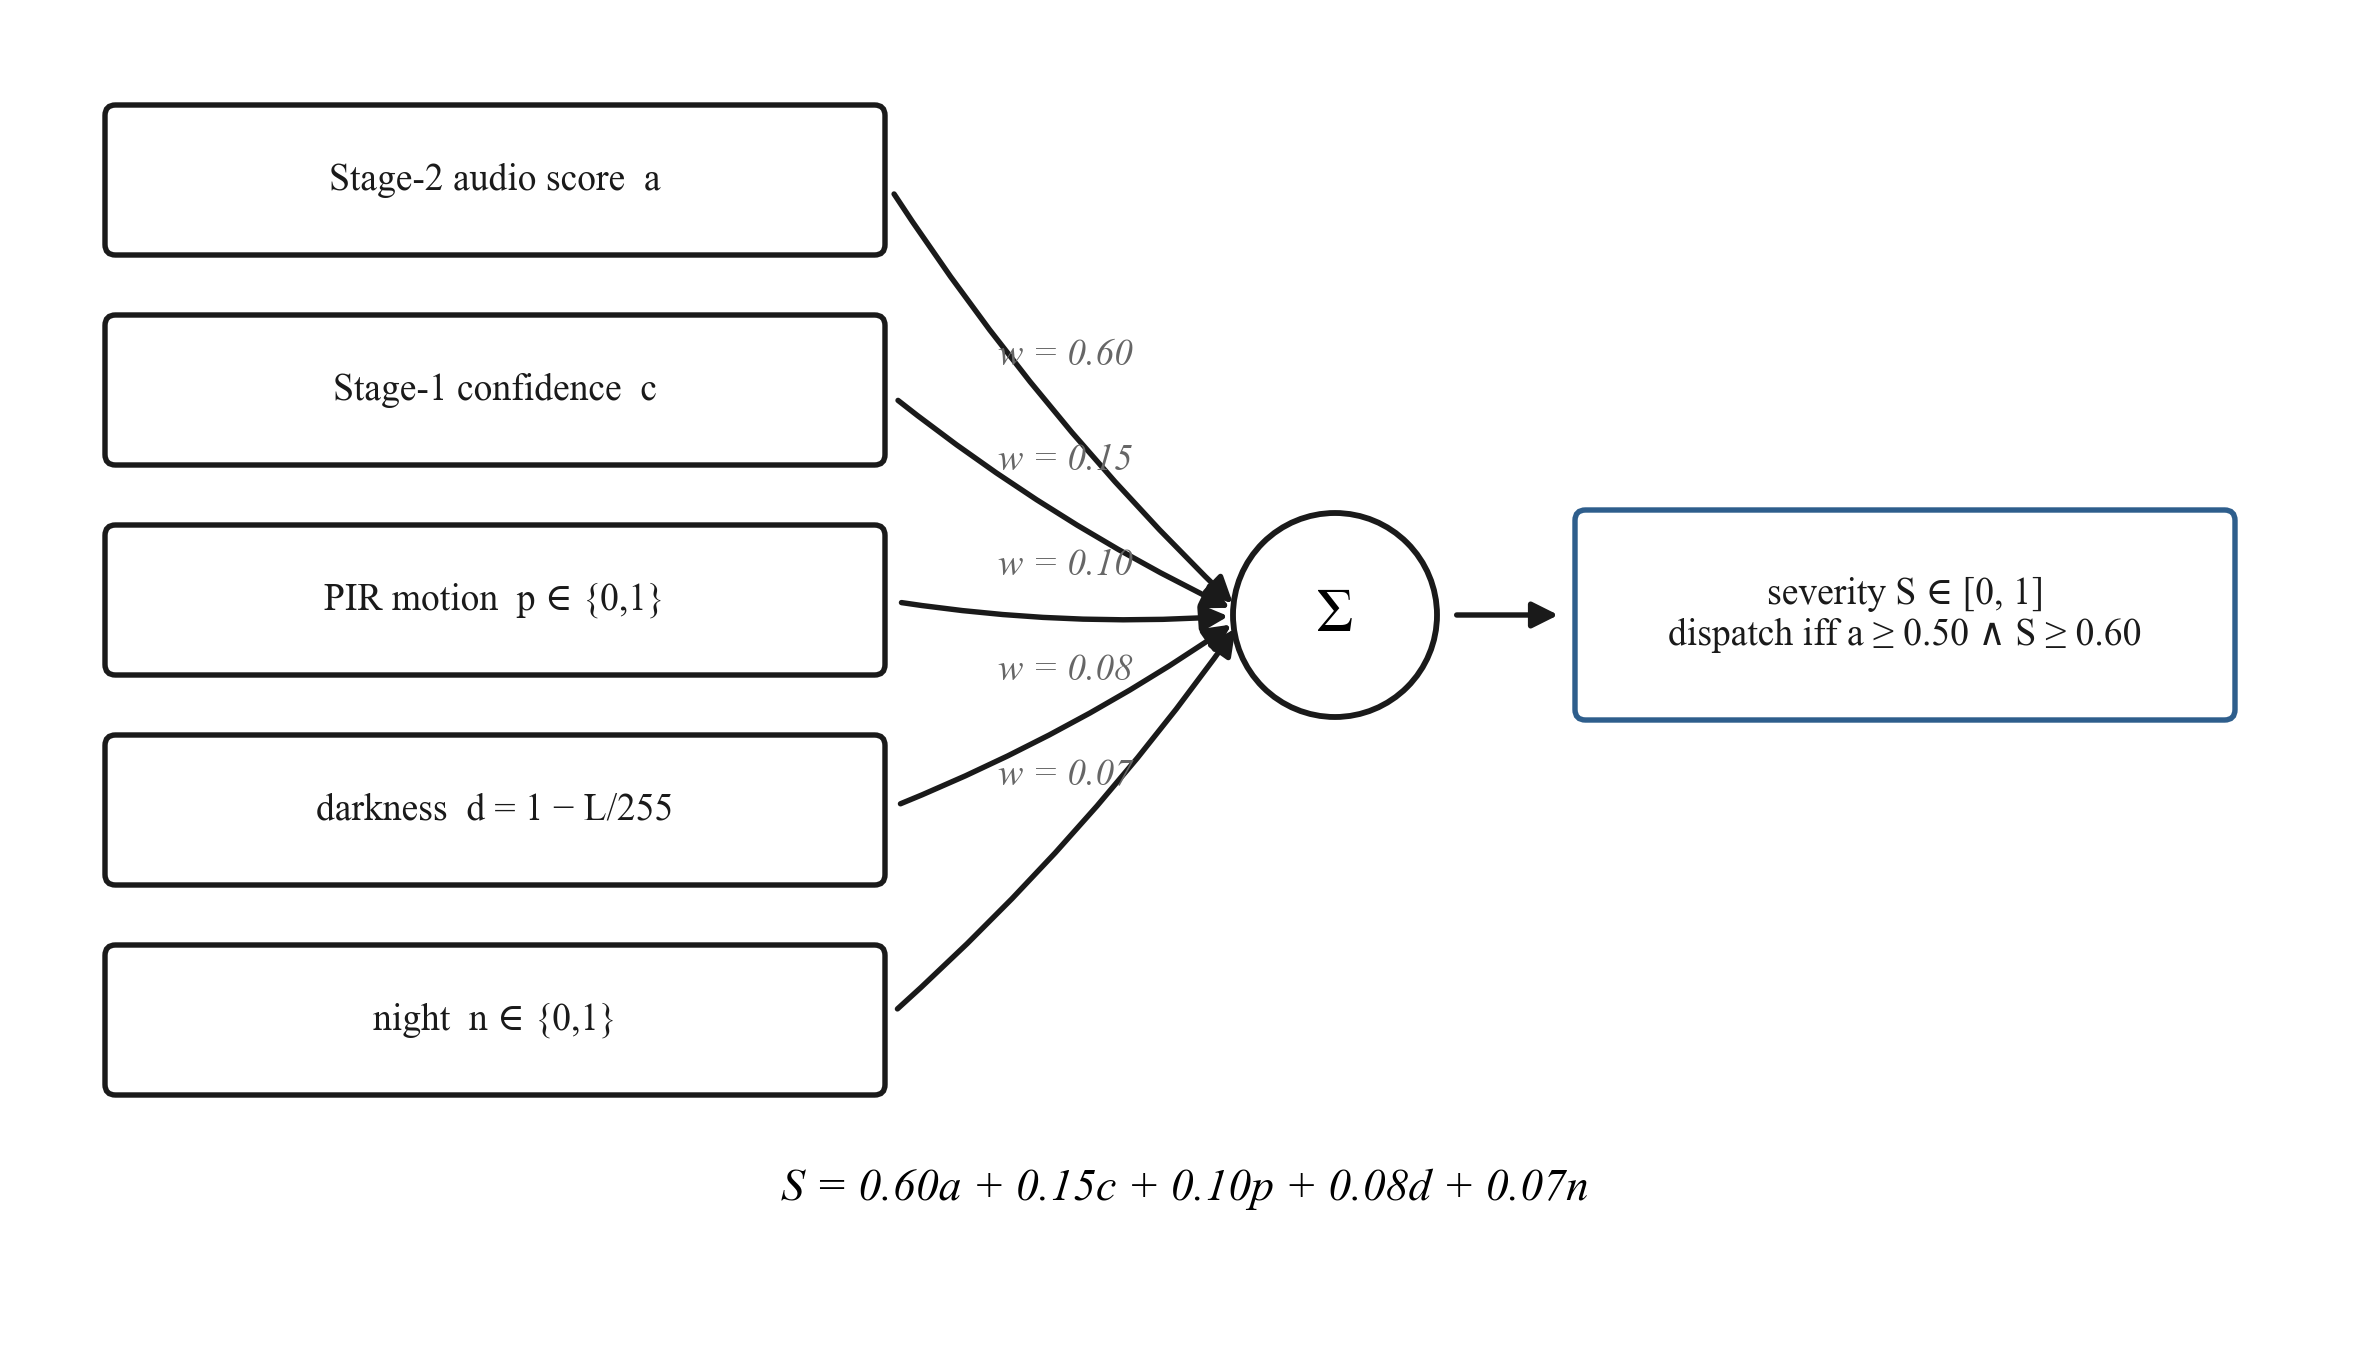
\includegraphics[width=\columnwidth]{fig7_fusion.png}
\caption{Evidence fusion at the hub: the Stage-2 audio score, Stage-1
confidence, PIR motion, darkness, and night indicator are combined with the
weights of \eqref{eq:fusion} and gated by the dual thresholds of
\eqref{eq:dispatch} before dispatch.}
\label{fig:fusion}
\end{figure}

\subsection{Degraded Path: Missing Clip}
\label{sec:degraded}

LoRa carries the alert but cannot carry audio
(Section~\ref{sec:alerting}), so Stage~2 depends on the ESP-NOW/WiFi clip
arriving. If no clip arrives within a bounded wait, the hub does not
silently drop the incident: it substitutes a degraded audio score
\begin{equation}
\label{eq:degraded}
a = 0.6\,c
\end{equation}
(the Stage-1 confidence at a haircut) and proceeds through fusion and
gating. In practice this means a low-confidence event without a clip will be
logged but not dispatched, while a very-high-confidence Stage-1 event may
still dispatch at reduced confidence. Multi-node
corroboration---raising confidence when neighboring nodes report the same
event---is identified as future work in this path.

\section{Secure Offline Alerting}
\label{sec:alerting}

\subsection{Threat Model}

The alert channel commands the launch of an autonomous aircraft. A forged
packet would dispatch a drone to an arbitrary location; a replayed packet
would re-dispatch it; an eavesdropped packet would reveal that (and where)
an incident is in progress. The protocol therefore provides confidentiality,
authenticity, and replay protection on every packet, under the constraint
that the whole message must fit comfortably in one LoRa frame at high
spreading factors.

\subsection{Packet Format}

Every alert is a fixed 25-byte packet (Table~\ref{tab:packet}), whose wire
layout is shown in Fig.~\ref{fig:packet}.

\begin{figure*}[!t]
\centering
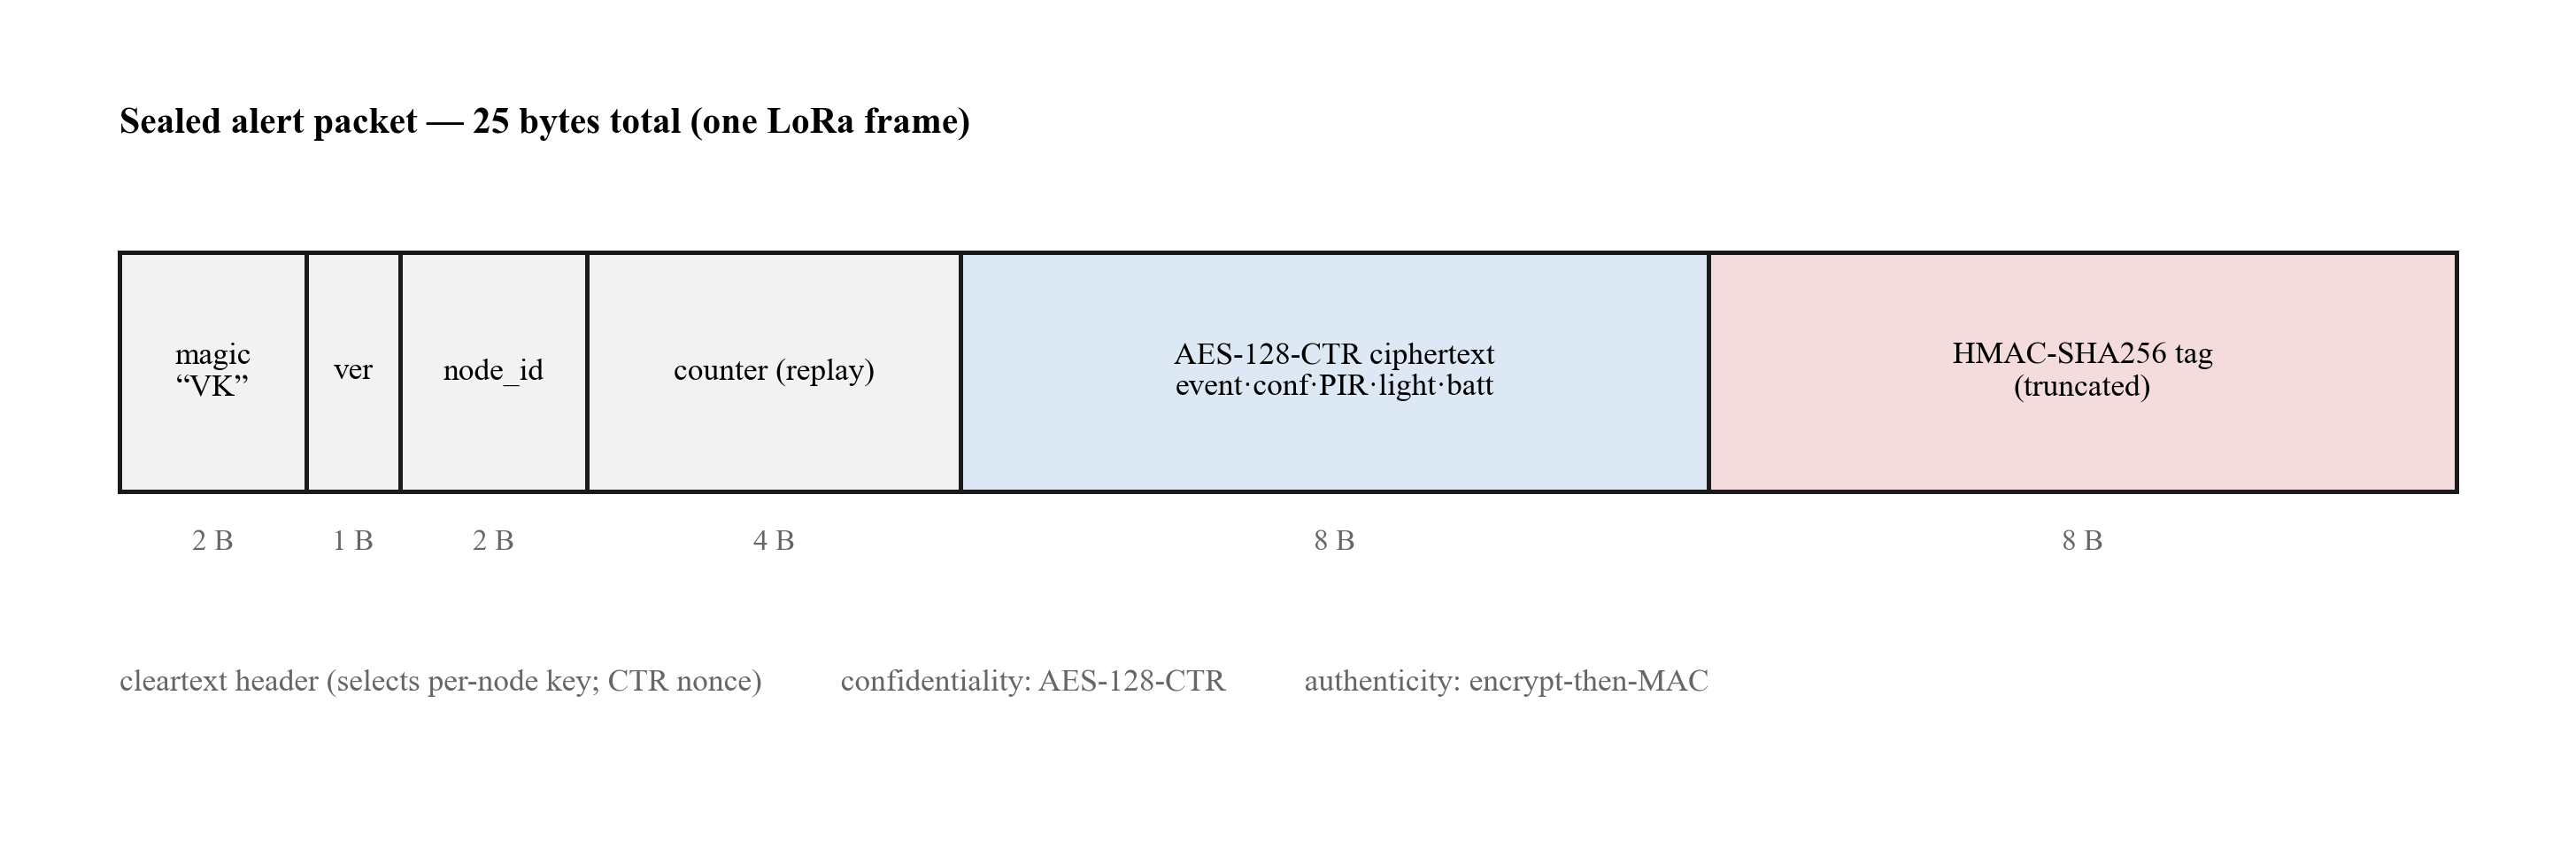
\includegraphics[width=\textwidth]{fig4_packet.png}
\caption{The 25-byte VanniKawachh alert packet: cleartext header (magic,
version, node ID, counter), 8-byte AES-128-CTR ciphertext, and 8-byte
truncated HMAC-SHA256 tag---sized to a single LoRa frame.}
\label{fig:packet}
\end{figure*}

\begin{table}[!t]
\caption{VanniKawachh LoRa Alert Wire Format (25 Bytes)}
\label{tab:packet}
\centering
\small
\begin{tabular}{@{}rrlp{3.0cm}@{}}
\toprule
Offset & Size & Field & Notes \\
\midrule
0 & 2 & Magic \texttt{``VK''} & Cleartext \\
2 & 1 & Version (1) & Cleartext \\
3 & 2 & \texttt{node\_id} (uint16, BE) & Cleartext; selects the per-node key \\
5 & 4 & \texttt{counter} (uint32, BE) & Cleartext; CTR nonce material and
replay check \\
9 & 8 & Payload ciphertext & AES-128-CTR \\
17 & 8 & MAC & HMAC-SHA256(node key, header $\parallel$ ciphertext),
truncated to 8 bytes \\
\bottomrule
\end{tabular}
\end{table}

The 8-byte encrypted payload carries: event class (1~=~scream,
2~=~help-keyword, 3~=~cry, 4~=~crash), Stage-1 confidence quantized to
0--255, PIR flag, LDR light level (0--255), node battery percentage, and
three reserved bytes.

\subsection{Cryptographic Construction}

Each node's key is derived from a single master key $K_m$ by keyed
hashing~\cite{rfc2104},
\begin{equation}
\label{eq:keyderivation}
K_n = \mathrm{HMAC\text{-}SHA256}\bigl(K_m,\ \text{``node:''} \parallel
n\bigr)[0{:}16],
\end{equation}
so provisioning a new node requires only the master key and an assigned ID
$n$, and compromise of one node's key does not reveal the master key or any
sibling key. Confidentiality is provided by AES-128~\cite{fips197} in CTR
mode: the plaintext payload $P$ is encrypted as
\begin{equation}
\label{eq:ctr}
C = P \oplus E_{K_n}(\mathrm{IV}),
\end{equation}
where the 16-byte counter block IV is built from the cleartext header
(magic $\parallel$ version $\parallel$ node\_id $\parallel$ counter), which
is unique per packet as long as the per-node counter is monotonic.
Authenticity is provided by an encrypt-then-MAC tag over the header and
ciphertext,
\begin{equation}
\label{eq:mac}
\tau = \mathrm{HMAC\text{-}SHA256}\bigl(K_n,\ \mathit{header} \parallel
C\bigr)[0{:}8],
\end{equation}
verified before decryption with a constant-time
comparison~\cite{rfc2104}. The hub persists the last accepted counter per
node, and a packet is accepted only when
\begin{equation}
\label{eq:accept}
\tau\ \text{valid} \;\wedge\; \mathit{counter} >
\mathit{counter}_{\mathrm{last}}.
\end{equation}
Under \eqref{eq:mac}, a forger without $K_n$ succeeds against the 64-bit
truncated tag with probability $2^{-64}$ per attempt---negligible at LoRa
frame rates. Packets with an unknown \texttt{node\_id}, a failed MAC, a
stale counter, or a malformed length are dropped and logged. All of these
rejection behaviors---tampered MAC, replayed counter, unknown node---are
pinned by automated tests.

\subsection{Why LoRa, and Why the Audio Travels Separately}

LoRa's link budget comes from spreading: each symbol carries $\mathit{SF}$
bits over a chirp of duration
\begin{equation}
\label{eq:symbolduration}
T_s = \frac{2^{\mathit{SF}}}{\mathit{BW}},
\end{equation}
so higher spreading factors buy sensitivity at the cost of airtime. The
receiver sensitivity floor is
\begin{equation}
\label{eq:sensitivity}
S_{\mathrm{dBm}} = -174 + 10\,\log_{10}(\mathit{BW}) + \mathit{NF} +
\mathit{SNR}_{\min},
\end{equation}
where $\mathit{NF}$ is the receiver noise figure and $\mathit{SNR}_{\min}$
the demodulation threshold for the chosen SF; at SF9--SF12 over
$\mathit{BW} = 125$~kHz this reaches below $-120$~dBm, which is what yields
multi-kilometre range from milliwatt nodes. The same trade caps throughput:
effective LoRa throughput at usable range is roughly 1--5.5~kbps. Applying
the standard LoRa time-on-air expression from the Semtech SX127x
datasheet~\cite{sx1278} to the 25-byte sealed alert at SF9, BW 125~kHz, CR
4/5, explicit header with CRC gives $\approx$0.21~s on air, whereas a 4~s
verification clip ($\approx$128~kB) at $\approx$5.5~kb/s effective would
occupy the channel for minutes---over three minutes even under ideal
conditions. This is the quantitative justification for the split: the
\emph{alert} travels over LoRa with no SIM or cellular dependency, delivered
essentially instantly at ranges of the 5--10~km class in open terrain (to be
measured for our deployment in Phase~2), while the 4~s \emph{verification
clip} travels over ESP-NOW/WiFi ($\sim$250~kbps, hundreds of metres
line-of-sight) to the hub. The alert path is the safety-critical one and has
no dependency on the clip path; if the clip is lost, the degraded-score path
of Section~\ref{sec:degraded} applies. The LoRaWAN
specification~\cite{lorawan} documents the underlying modulation and
regional parameters; the prototype uses raw LoRa point-to-point framing
rather than a full LoRaWAN network stack, since each node speaks only to its
own hub.

\section{Safety-Verified Autonomous Response}
\label{sec:safety}

The response tier is where a software error stops being a bug and becomes a
hazard to people on the ground. The flight stack therefore treats the
autopilot as an \emph{unreliable command sink} and enforces safety as a set
of structural invariants in the companion computer, above and in addition to
the autopilot firmware's own failsafes. The mission executor's
thirteen-state machine, within which every mechanism of this section
operates, is shown in Fig.~\ref{fig:statemachine}. The mechanisms in this
section are the subject of two patent applications in preparation.

\begin{figure*}[!t]
\centering
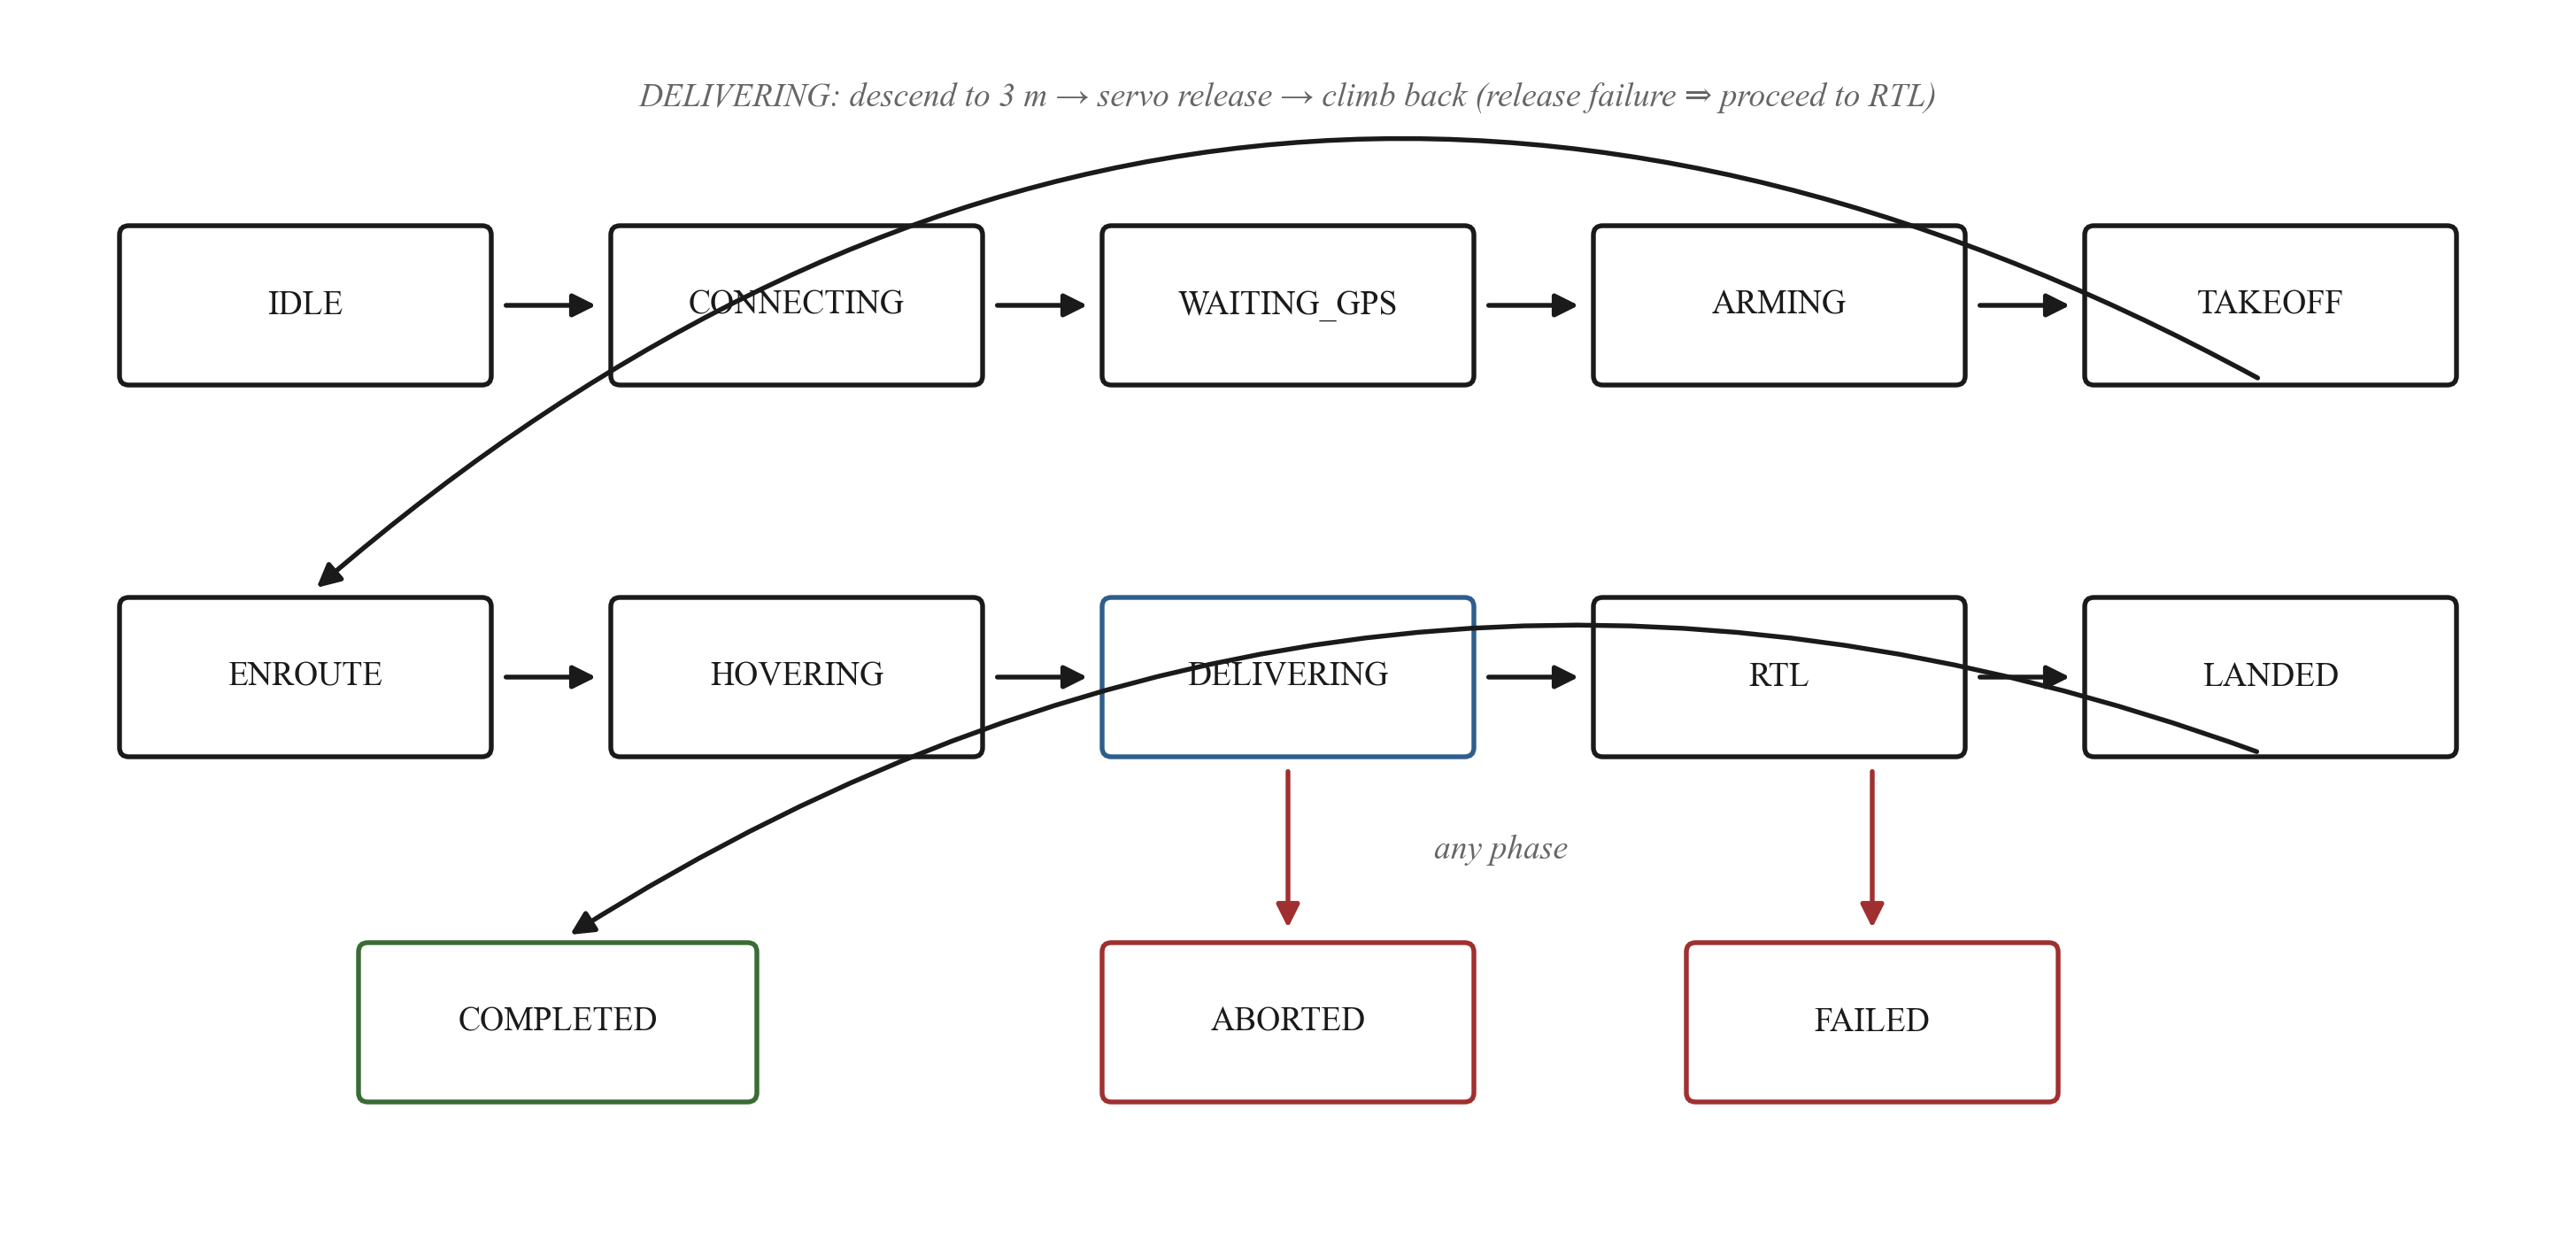
\includegraphics[width=\textwidth]{fig5_state_machine.png}
\caption{The 13-state mission finite-state machine, from IDLE through
TAKEOFF, ENROUTE, HOVERING, and DELIVERING to RTL and LANDED, with the
abnormal-termination paths into ABORTED and FAILED.}
\label{fig:statemachine}
\end{figure*}

\subsection{Verified Flight-Mode Delivery}

Autopilot firmware may silently reject or drop a flight-mode change: the
client library reports success while the autopilot remains in its previous
mode. We observed this empirically on an ArduCopter SITL autopilot, where a
GUIDED-mode request was reported accepted while the vehicle remained in
STABILIZE, causing the subsequent takeoff command to be silently ignored. In
a human-piloted system an operator notices and retries; in an autonomous
system there is no operator---and the same unverified pathway carries the
\emph{emergency} commands (RTL, LAND).

All mode transitions therefore flow through a single verified setter. It
issues the transition through the high-level client interface, then enters a
confirmation loop bounded by a timeout (10--15~s): on each iteration it
reads the flight mode the autopilot itself reports in its HEARTBEAT-derived
telemetry. Until the reported mode matches, it re-issues the command at a
$\sim$700~ms interval through \emph{layered protocol encodings}: a MAVLink
\texttt{COMMAND\_LONG} carrying \texttt{MAV\_CMD\_DO\_SET\_MODE} with the
resolved custom-mode identifier, a MAVLink \texttt{SET\_MODE} message, and
the high-level interface again. Mode-set requests are idempotent, so
redundant issuance is harmless; because confirmation is read from the
autopilot's own report, no client-side state is trusted. A transition is
treated as delivered \emph{only} upon telemetry confirmation.

\subsection{Cross-Action Emergency Fallback}

If an emergency transition cannot be confirmed within the timeout, the
executor substitutes the alternative emergency action through the same
verified routine: an unconfirmable RTL becomes a LAND command, and vice
versa. The rationale is that some \emph{confirmed} recovery action is
preferable to an optimal but unconfirmed one. One asymmetry is enforced: a
LAND demand is never downgraded to RTL.

\subsection{Landing-Interlocked Serial Dispatch}

Missions are executed strictly serially from a bounded priority queue, and
the queue maintains the invariant that \emph{no mission ever begins against
an airborne vehicle}, via two cooperating mechanisms. First, the
\textbf{abort guarantee}: every abnormal-termination path---failsafe action,
operator recall, or unhandled exception with the vehicle airborne---commands
its recovery mode through the verified setter and then blocks, polling
telemetry, until the vehicle reports disarmed at near-zero relative altitude
(bounded at 240~s) before control returns to the queue worker. Second, the
\textbf{pre-flight interlock}: on dequeuing a mission, the executor reads
the vehicle's armed flag and, if armed, waits up to 120~s for disarm;
failing that, the mission is failed without a single arming or takeoff
command being issued. The first mechanism makes violation improbable; the
second makes it impossible.

\subsection{Failsafe Arbiter}

A supervisory thread polls vehicle telemetry at 1~Hz throughout the mission,
evaluating named hazard conditions: battery against a low threshold (demands
RTL) and a critical threshold (demands LAND), GPS fix validity, geofence
distance from home, mission wall-clock duration, MAVLink heartbeat
staleness, and per-leg navigation progress (stall detection). The arbiter
maintains a single demanded action over the ordered set NONE $<$ RTL $<$
LAND with three disciplines.
\begin{itemize}
\item \textbf{Debounce.} GPS loss fires only after $N$ consecutive anomalous
1~Hz samples ($N = 3$ by default), with any valid sample resetting the
count---a single corrupted sample never lands the aircraft. GPS loss demands
LAND rather than RTL because a home-bound trajectory is not navigable
without positioning.
\item \textbf{Severity ordering.} The demanded action is monotone
non-decreasing within a mission: a LAND demand is never replaced by RTL.
Escalation is honored \emph{mid-recovery}---the RTL phase re-reads the
demand on every iteration and, if it has escalated (e.g., battery fell from
low to critical during the return), abandons the return and commands LAND
through the verified setter.
\item \textbf{Fire-once event discipline.} Each named hazard emits one event
per mission, with re-emission accepted only when it escalates the demanded
action, keeping the incident record free of duplicate floods from persistent
conditions.
\end{itemize}

The executor consults the arbiter inside every blocking loop and at every
phase boundary, so no flight phase can outlive a demanded recovery by more
than one polling interval. Fig.~\ref{fig:interlock} summarizes how the
mechanisms of this section chain into five successive gates---geofence
validation, the pre-flight landing interlock, verified mode delivery,
continuous failsafe arbitration, and the bounded abort guarantee---each of
which must pass before or during any flight activity.

\begin{figure*}[!t]
\centering
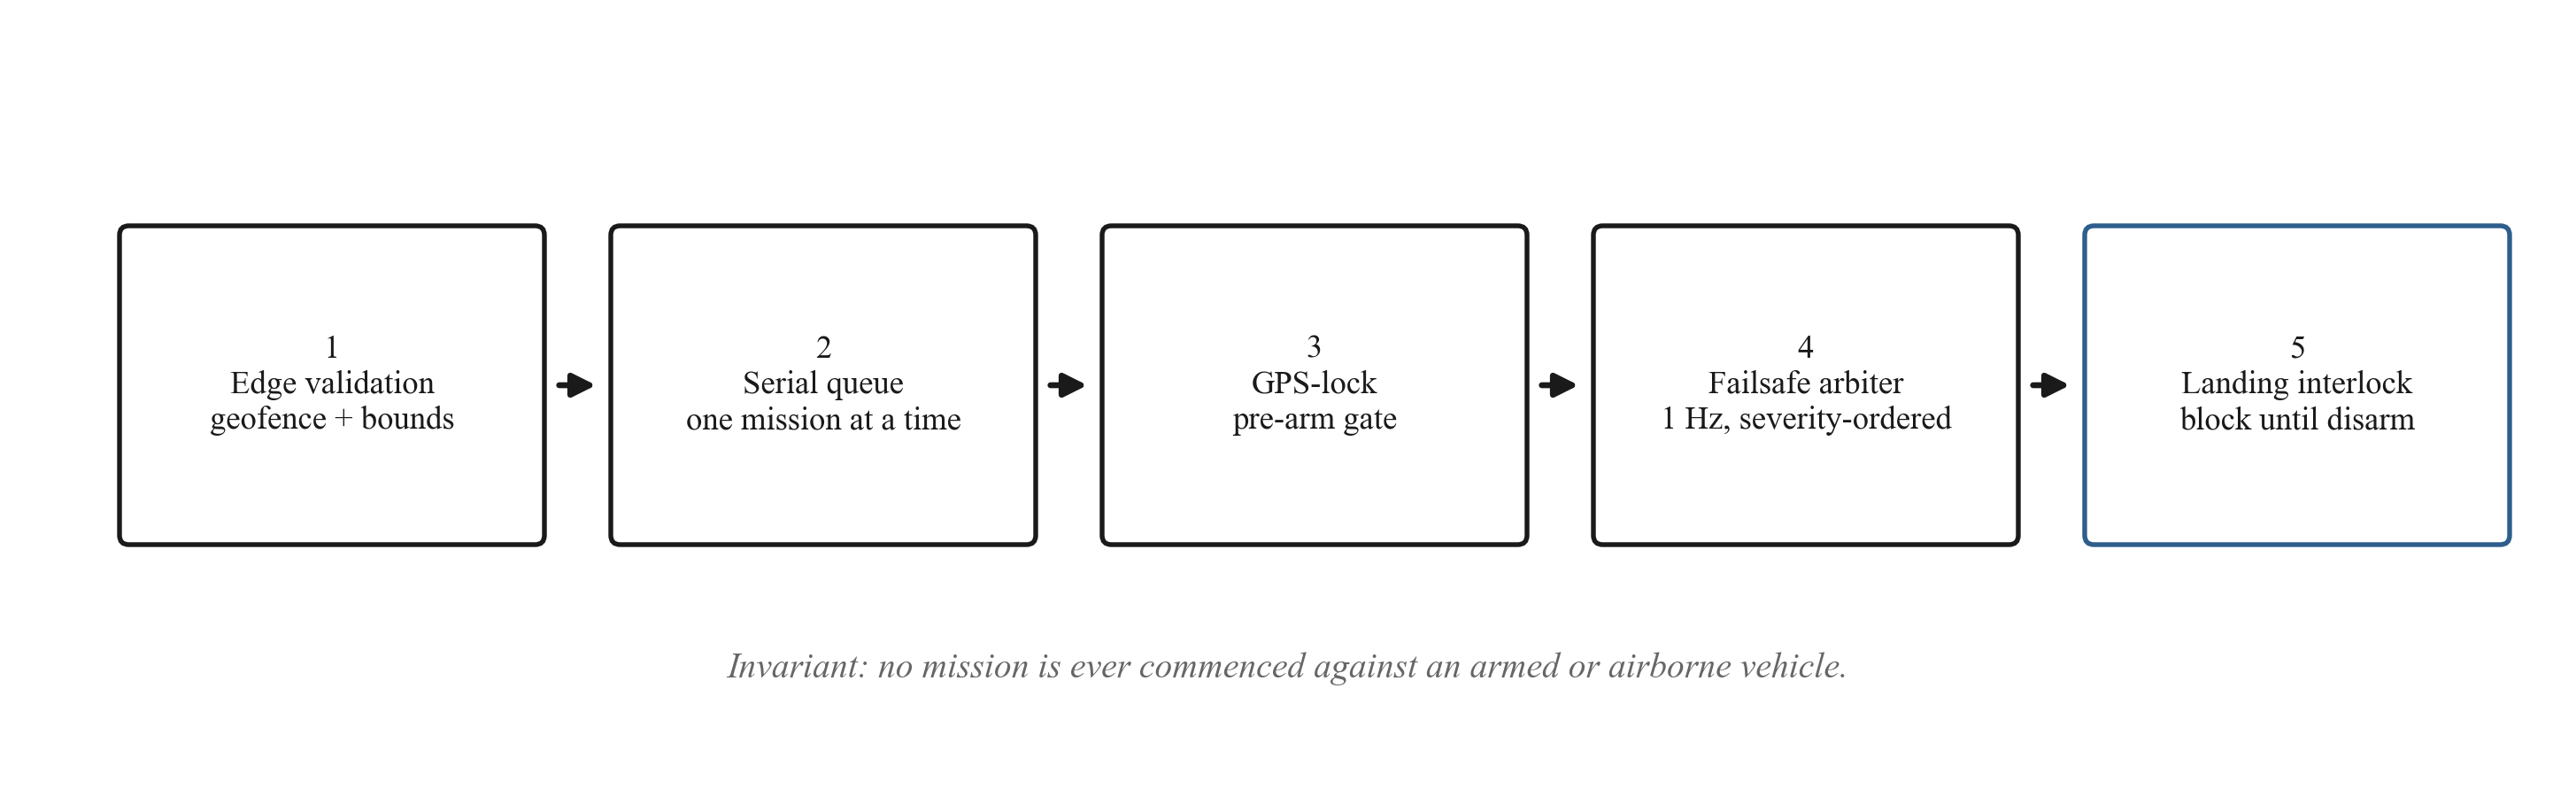
\includegraphics[width=\textwidth]{fig6_interlock.png}
\caption{The five-gate safety chain protecting every dispatch: edge geofence
validation, landing interlock, telemetry-verified mode delivery, the 1~Hz
failsafe arbiter, and the abort guarantee that blocks until the vehicle is
disarmed on the ground.}
\label{fig:interlock}
\end{figure*}

\subsection{Geofence Validation at the Network Edge}

The trigger interface validates every dispatch target and every in-flight
waypoint against a software geofence centred on home, rejecting
non-compliant requests with a client error \emph{before any flight
activity}---converting what would otherwise be an in-flight abort into a
pre-flight validation error. All great-circle distances in the stack---the
geofence radius check, arrival detection against the 5~m waypoint tolerance,
and ETA estimation---are computed with the haversine formula,
\begin{equation}
\label{eq:haversine}
d = 2R \arcsin\!\sqrt{\sin^2\!\frac{\Delta\varphi}{2} +
\cos\varphi_1 \cos\varphi_2 \sin^2\!\frac{\Delta\lambda}{2}},
\end{equation}
with $R = 6371$~km, where $(\varphi_1, \lambda_1)$ and $(\varphi_2,
\lambda_2)$ are the two latitude/longitude pairs; at mission ranges of a few
kilometres its error is far below the GPS error itself. The software fence
is secondary to the autopilot's own hardware-level \texttt{FENCE\_*}
enforcement, which is also configured on real airframes.

\subsection{DELIVERING: The Payload Phase}

For VanniKawachh missions the state machine inserts a DELIVERING phase
between HOVERING and RTL. The drone descends over the incident point to the
configured drop altitude ($\leq$3~m), commands the SG90 release hook through
the flight controller with \texttt{MAV\_CMD\_DO\_SET\_SERVO} on an AUX
output channel, and climbs back to cruise altitude. The 3~m ceiling is set
by simple ballistics: a kit released from height $h$ falls for
\begin{equation}
\label{eq:falltime}
t = \sqrt{2h/g} \approx 0.78~\mathrm{s} \quad \text{at } h = 3~\mathrm{m},
\end{equation}
during which a horizontal wind of speed $v_w$ drifts it approximately
\begin{equation}
\label{eq:drift}
x \approx v_w\,t \approx 1.6~\mathrm{m} \quad \text{at } v_w =
2~\mathrm{m/s},
\end{equation}
so even in a moderate breeze the kit lands within reach of the victim,
while releasing from cruise altitude would multiply both the drift and the
impact energy. Two rules are enforced: the kit is released only from a
$\leq$3~m hover, and a \emph{failed release is reported but never blocks the
mission}---the drone proceeds to RTL either way, never loitering on a failed
drop. The camera recorder runs across HOVERING and DELIVERING, writing an
MP4 tagged with the mission ID as the evidence artifact; on machines without
a camera (SITL, development hosts) it is a no-op stub, so the mission flow
is identical.

\subsection{Onboard State Estimation}

The position and velocity estimates that GUIDED flight, arrival detection,
and every failsafe check consume are produced by the autopilot's extended
Kalman filter, which fuses GNSS, IMU, barometer, and magnetometer
measurements. At each step the filter propagates the state through the
vehicle dynamics model,
\begin{equation}
\label{eq:ekfpredict}
\hat{x}_k^{-} = f(\hat{x}_{k-1}, u_k), \qquad
P_k^{-} = F P_{k-1} F^{\mathsf{T}} + Q,
\end{equation}
and corrects it with the incoming measurement $z_k$ via the Kalman gain,
\begin{equation}
\label{eq:ekfupdate}
\begin{aligned}
K_k &= P_k^{-} H^{\mathsf{T}} \bigl(H P_k^{-} H^{\mathsf{T}} +
R\bigr)^{-1}, \\
\hat{x}_k &= \hat{x}_k^{-} + K_k \bigl(z_k - h(\hat{x}_k^{-})\bigr).
\end{aligned}
\end{equation}
The companion computer deliberately treats this estimate as the single
source of truth---the verified mode setter, the arbiter, and the landing
interlock all read the autopilot's EKF-derived telemetry rather than
maintaining any client-side dead reckoning of their own.

\section{Experimental Results}
\label{sec:results}

All results in this section are software-in-the-loop or automated-test
results, obtained with the ArduPilot SITL simulator~\cite{ardupilot} in
place of a physical airframe. We state explicitly what each number is and is
not; hardware measurements pending as of this writing are enumerated in
Section~\ref{sec:pending}.

\subsection{SITL Flight Validation}

The acceptance harness spawns an ArduCopter SITL instance and the full
flight stack as child processes, dispatches a mission over the real HTTP
trigger interface, and monitors live telemetry throughout. The results are
as follows.
\begin{itemize}
\item \textbf{8 of 8 acceptance checks passed}: API health and vehicle
connection, mission acceptance, arming and takeoff, cruise-altitude
attainment, target arrival within tolerance, hover phase, RTL, and
landed/disarmed completion.
\item \textbf{Terminal accuracy of 0.4~m} against the configured 5~m
waypoint tolerance---the minimum distance-to-target observed during the
approach.
\item \textbf{Complete autonomous mission in 328~s} wall-clock, from trigger
POST to landed-and-disarmed.
\item \textbf{Battery drained from 100\% to 32\%} over the run with
\textbf{zero false failsafe activations}: neither the low-battery nor any
other failsafe fired spuriously during a nominal mission, while remaining
armed at the 1~Hz polling cadence throughout.
\end{itemize}

\subsection{Unit Verification}

A suite of \textbf{68 automated tests} pins the safety and security
properties claimed in
Sections~\ref{sec:acoustic}--\ref{sec:safety}: failsafe thresholds, debounce
behavior (no trigger at $N-1$ anomalous GPS samples, trigger at $N$, count
reset on recovery), severity escalation including LAND-over-RTL mid-return
and refusal to downgrade LAND; queue landing interlocks; alert-packet
seal/unseal round-trips, tamper rejection (corrupted MAC), and replay
rejection (stale counter); fusion scoring; pipeline dispatch gating (no
dispatch below threshold); and obstacle keep-out route geometry. Every
safety claim written in this paper is pinned by at least one of these tests
or by the acceptance harness.

\subsection{End-to-End Chain Rehearsal (Phase 0)}
\label{sec:rehearsal}

A full-chain rehearsal exercised every architectural interface with zero
hardware: a simulated node event was sealed into the 25-byte packet format,
delivered to the hub pipeline, authenticated and decrypted, verified and
fused (fused severity 0.88, priority \emph{high}), resolved against the node
registry, and dispatched as an HTTP trigger; the SITL drone then flew the
mission autonomously---takeoff, transit, hover-observe with the (no-op)
evidence recorder, descent to 3.1~m for payload release, simulated servo
release, return, and landing, with the state machine terminating in
COMPLETED. Fig.~\ref{fig:missionprofile} shows the rehearsal's altitude
profile, with the descent to the 3.1~m kit-release point clearly visible
between the hover window and the return leg.

\begin{figure*}[!t]
\centering
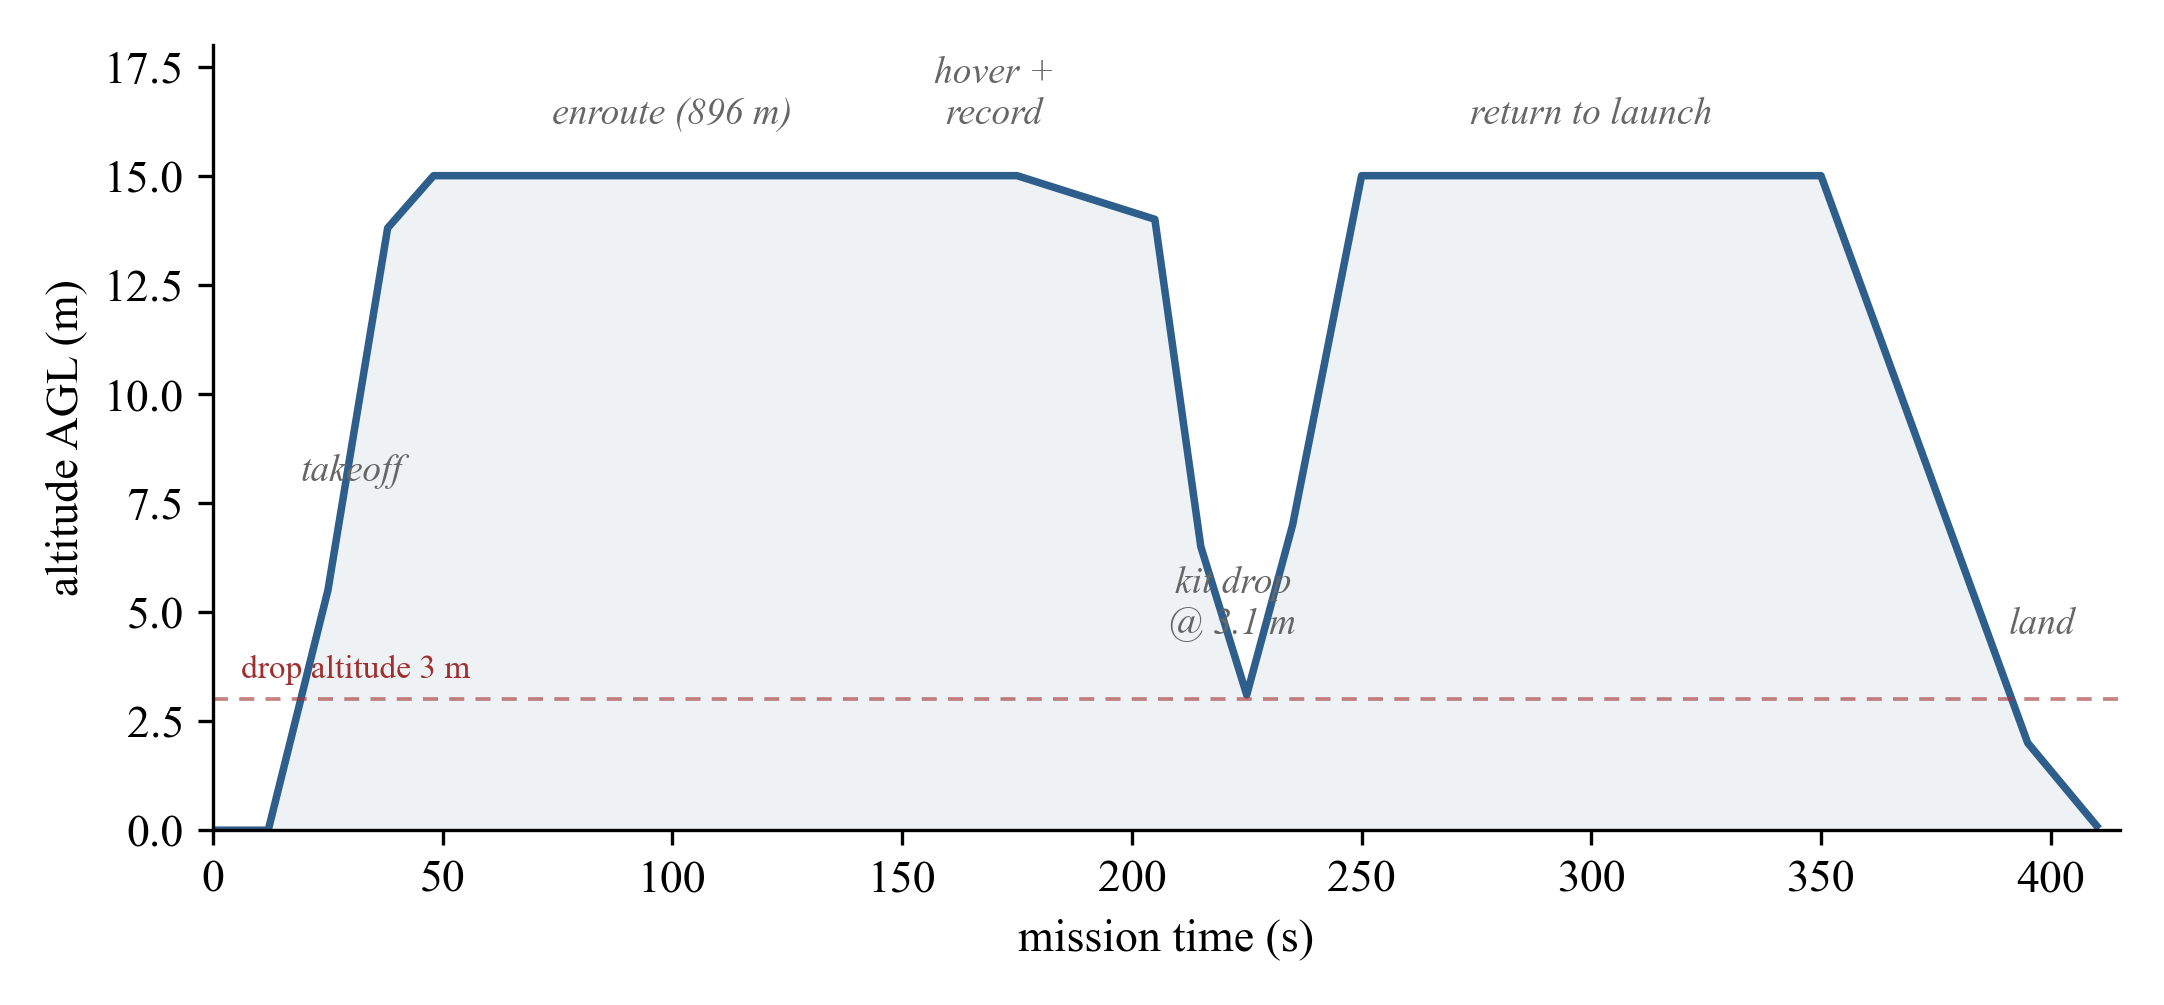
\includegraphics[width=\textwidth]{fig8_mission_profile.png}
\caption{Altitude profile of the Phase-0 full-chain rehearsal mission:
takeoff to cruise, transit, hover-observe, descent to the 3.1~m kit release,
climb-out, and return to launch, completing in 328~s.}
\label{fig:missionprofile}
\end{figure*}

This rehearsal validates the \emph{integration contract} of the whole chain:
packet format, registry lookup, gating thresholds, dispatch payload, and
mission state sequence. Two caveats apply and are stated plainly: the
rehearsal's Stage-2 scoring used the hub's energy-heuristic fallback backend
rather than PANNs (which deploys on the physical Pi~5), and the simulated
node used the calibrated heuristic Stage-1 screen rather than a trained TFLM
model. For transparency, the fallback scorer that produced the rehearsal's
audio score is fully specified: over the clip samples $x[n]$ it computes the
root-mean-square level
\begin{equation}
\label{eq:rms}
\mathrm{RMS} = \sqrt{\frac{1}{N} \sum_{n} x^{2}[n]},
\end{equation}
the spectral centroid
\begin{equation}
\label{eq:centroid}
C = \frac{\sum_{f} f\,|X(f)|}{\sum_{f} |X(f)|},
\end{equation}
and an envelope-burstiness term, combining them as
\begin{equation}
\label{eq:heuristic}
\begin{split}
\text{score} = {}& 0.45\,\min(1, \mathrm{RMS}/0.15) \\
& + 0.35\,\operatorname{clip}\!\bigl((C - 400)/1600,\ 0,\ 1\bigr) \\
& + 0.20\,\text{burstiness}.
\end{split}
\end{equation}
Equation~\eqref{eq:heuristic} is a labeled development stand-in---loud,
high-centroid, bursty audio scores high---and every result produced with it
is marked as such; it is not a claim of detection accuracy. The rehearsal is
therefore evidence of architectural correctness, not of acoustic detection
accuracy.

\subsection{Evaluation in Progress}
\label{sec:pending}

The following measurements require physical hardware and are scheduled in
the build plan; none are claimed in this paper.

\begin{table}[!t]
\caption{Pending Hardware Measurements (Evaluation in Progress)}
\label{tab:pending}
\centering
\small
\begin{tabular}{@{}p{3.4cm}lp{2.5cm}@{}}
\toprule
Measurement & Phase & Status \\
\midrule
Stage-1 TFLM model accuracy/recall on scream + keyword corpora & Phase 1 &
Model training pending; heuristic stand-in deployed \\
Stage-1 on-device latency on ESP32-S3 ($<$50~ms target) & Phase 1 & Not yet
measured \\
Outdoor detection distance vs.\ SNR (INMP441, street noise) & Phase 1 & Not
yet measured \\
Stage-2 PANNs latency on Raspberry Pi~5 & Phase 1 & Not yet measured \\
End-to-end false-positive rate on real street noise & Phases 1--2 & Not yet
measured \\
LoRa range (urban/open) and packet loss vs.\ spreading factor & Phase 2 &
Not yet measured \\
Physical flight replication of SITL results (VLOS field trials) & Phases
3--4 & Not yet flown \\
\bottomrule
\end{tabular}
\end{table}

Accordingly, this paper's validated contribution is best characterized as
\emph{architecture + safety framework + software-in-the-loop validation of
the response chain}, with the acoustic pipeline's accuracy figures deferred
to the hardware evaluation phases (Table~\ref{tab:pending}).

\section{Discussion}
\label{sec:discussion}

\subsection{Privacy by Construction}

A pole-mounted microphone network invites legitimate privacy concern, and
VanniKawachh addresses it structurally rather than by policy. There is no
continuous recording and no continuous transmission: audio is processed in
place on the node and discarded frame-by-frame unless Stage~1 fires. Only
event-triggered clips of at most 5~s ever leave a node, and the alert itself
is encrypted. The node stores no audio at rest, and the hub retains clips
only as incident evidence. Because nodes carry no GPS and no identity beyond
a numeric ID, a captured node reveals its own derived key but neither the
master key nor any location data beyond what is physically observable.

This structural posture is also the system's answer to India's Digital
Personal Data Protection Act, 2023~\cite{dpdp2023}, which requires purpose
limitation, data minimization, and security safeguards for digital personal
data. VanniKawachh's design maps directly onto those obligations: on-device
processing means ambient conversation is never collected in the first place;
the only personal data that ever exists is an event-triggered clip of at
most 5~s, retained solely as incident evidence for a defined safety purpose;
and everything in transit is encrypted (AES-128-CTR with authenticated
packets on the alert path). A production deployment would still require a
documented lawful basis, retention schedule, and notice regime under the Act
and its rules, but the architecture ensures compliance is a matter of
process on top of a minimizing design, not remediation of an over-collecting
one.

\subsection{Regulatory Context}

UAS operations in India are governed by The Drone Rules, 2021, notified as
G.S.R. 589(E) by the Ministry of Civil Aviation~\cite{dronerules2021}. The
Rules require every UAS to be registered on the DGCA's Digital Sky platform
and issued a Unique Identification Number, and they partition Indian
airspace into green, yellow, and red zones: operations up to 400~ft in green
zones require no prior permission, yellow zones require air-traffic-control
clearance, and red zones are no-fly except by central-government exception.
Prototype flight operations are designed to sit in the least-restrictive
cell of this framework: the airframe is registered on Digital Sky, and all
test flights are conducted in green-zone airspace within visual line of
sight (VLOS) over open private ground with an RC safety pilot holding
override authority at all times. Fully autonomous
beyond-visual-line-of-sight (BVLOS) response---the operationally interesting
deployment mode---is described here as a \emph{supervised pilot-program
pathway} contingent on regulatory approval (the Rules and subsequent DGCA
BVLOS experiment schemes provide exactly such a pathway), not as a
capability of the prototype. The architecture anticipates this: the police
dashboard already provides the human-supervision surface (live telemetry,
incident log, and a recall endpoint that is the operator's only
override---there is deliberately no joystick).

The radio links sit within India's licence-exempt spectrum framework
administered by the Wireless Planning and Coordination (WPC) Wing of the
Department of Telecommunications. The prototype's SX1278 transceivers
operate as low-power short-range devices at 433~MHz; a production deployment
would migrate to the delicensed 865--867~MHz band~\cite{wpc865}, where
higher transmit power is permitted without an operating licence and where
Indian LoRa deployments conventionally operate, improving both link budget
and regulatory headroom. Neither band requires a spectrum licence at the
power levels used, which preserves the system's core property of
deployability without any telecom-operator dependency.

\subsection{Limitations}

Beyond the pending measurements of Table~\ref{tab:pending}, several
limitations are acknowledged. (1)~The fusion weights and dispatch thresholds
are prototype values pending calibration against bench data; the false-alarm
behavior of the full two-stage pipeline in real acoustic environments is
the single most important unvalidated property. (2)~The 25-byte alert's
8-byte truncated MAC trades authentication strength for frame budget; at
LoRa alert rates, brute-force forgery is impractical, but the trade-off
should be revisited if the channel is ever widened. (3)~The hub is a single
point of failure per locality; node-to-node relaying and hub redundancy are
not yet designed. (4)~The clip path (ESP-NOW/WiFi) has far shorter range
than the alert path, so nodes far from the hub will operate predominantly in
the degraded-score mode. (5)~SITL validates control logic, not aerodynamics,
wind, GPS multipath, or real sensor noise; physical flight trials may
surface effects the simulator does not model. (6)~One drone serves one
locality serially; concurrent incidents queue by priority rather than being
served in parallel.

\section{Conclusion and Future Work}
\label{sec:conclusion}

VanniKawachh demonstrates that a women-safety system need not place any
burden---device, charge, coverage, or action---on the woman it protects. The
architecture couples infrastructure-mounted two-stage acoustic sensing to an
offline, cryptographically sealed alert channel and an autonomous aerial
first-response layer whose safety rests on verified command delivery,
severity-ordered failsafe arbitration, and a landing-interlocked dispatch
queue. Software-in-the-loop validation shows the complete chain---from
sealed alert to first-aid drop---functioning end-to-end with 8/8 acceptance
checks and 0.4~m terminal accuracy, and 68 automated tests pin every stated
safety property.

Future work proceeds on two fronts. Near-term hardware evaluation
(Table~\ref{tab:pending}) will supply the acoustic accuracy, latency, range,
and false-alarm figures this paper deliberately declines to estimate. Beyond
that, four extensions are planned: live video streaming from the drone to
the police dashboard (RTSP/WebRTC); OpenCV-based victim detection and
tracking during hover; multi-node time-difference-of-arrival (TDOA)
localization to position events between poles rather than at them; and a
city-scale node mesh with hub federation. The flight-safety mechanisms of
Section~\ref{sec:safety} are the subject of two Indian patent applications
in preparation.

\section*{Acknowledgment}

The authors thank Dr.~Aditya Turankar, Department of Computer Science and
Engineering, G H Raisoni College of Engineering, Nagpur, for guidance
throughout this work.

\begin{thebibliography}{99}

\bibitem{pavithra2026}
R. Pavithra, R. Ahalya, and C. Shuruthika, ``Discreet AI-powered women's
safety app with audio recognition and emergency automation,'' in \emph{Proc.
2026 IEEE Students Conf. Eng. Syst. (SCEECS)}, Bhopal, India, 2026, doi:
10.1109/SCEECS68810.2026.11430037.

\bibitem{kim2025}
Y. Kim, D. Jang, and S.-P. Lee, ``Robust scream detection and scream
temporal interval prediction using CNN-Transformer and windowing CNN,''
\emph{IEEE Access}, vol. 13, pp. 71374--71387, 2025, doi:
10.1109/ACCESS.2025.3556729.

\bibitem{sharma2025}
P. Sharma and T. J. Jebaseeli, ``Smart scream and panic detection system for
women using AI,'' in \emph{Proc. 2025 Int. Conf. Autom. Comput. Renew. Syst.
(ICACRS)}, 2025, pp. 1554--1559, doi: 10.1109/ICACRS67045.2025.11324333.

\bibitem{srimathi2025}
A. Srimathi, S. Jothi, and M. P. Sindhiya, ``Human scream detection and
analysis for crime reduction,'' in \emph{Proc. 2025 Int. Conf. Multidiscip.
Sci. Comput. Intell. (ICMSCI)}, Erode, India, 2025, pp. 1528--1534, doi:
10.1109/ICMSCI62561.2025.10894058.

\bibitem{bharathi2025}
P. S. Bharathi \emph{et al.}, ``A novel IoT enabled women safety system
design with emergency alert mechanism,'' in \emph{Proc. 2025 Int. Conf.
Future Technol. Syst. (ICFTS)}, 2025, pp. 1--7, doi:
10.1109/ICFTS62006.2025.11031774.

\bibitem{snehith2025}
R. Snehith, S. Saranya, and N. R. Reddy, ``A smart device for women safety
using IoT,'' in \emph{Proc. 2025 Int. Conf. Intell. Syst. Sci. (ICISS)},
2025, pp. 277--282, doi: 10.1109/ICISS63372.2025.11076270.

\bibitem{kim2024}
Y. Kim, D. Jang, and J. Lee, ``Development of scream detection system with
large-scale scream dataset,'' in \emph{Proc. 2024 Int. Conf. Inf. Commun.
Technol. Converg. (ICTC)}, Jeju, South Korea, 2024, pp. 590--593, doi:
10.1109/ICTC62082.2024.10826757.

\bibitem{fime2024}
A. A. Fime, M. Ashikuzzaman, and A. Aziz, ``Audio signal-based danger
detection using signal processing and deep learning,'' \emph{Expert Systems
with Applications}, vol. 237, art. no. 121646, Mar. 2024, doi:
10.1016/j.eswa.2023.121646.

\bibitem{hadkar2024}
R. V. Hadkar \emph{et al.}, ``An efficient IoT-enabled women safety
device,'' in \emph{Proc. 2024 Int. Conf. Autom. Comput. Renew. Syst.
(ICACRS)}, 2024, pp. 425--431, doi: 10.1109/ICACRS62842.2024.10841797.

\bibitem{uganya2023}
G. Uganya \emph{et al.}, ``Smart women safety device using IoT and GPS
tracker,'' in \emph{Proc. 2023 Int. Conf. Comput. Electron. Biomed. Syst.
(ICCEBS)}, Chennai, India, 2023, pp. 1--6, doi:
10.1109/ICCEBS58601.2023.10449302.

\bibitem{potturi2026}
S. Potturi \emph{et al.}, ``An SOS women safety device: Automatic emergency
alerts and geo-location sharing with GSM/GPS integration,'' in \emph{Proc.
2026 Int. Conf. Intell. Comput. Netw. Syst. (IC-ICNS)}, Bhubaneswar, India,
2026, pp. 1--6, doi: 10.1109/IC-ICNS68863.2026.11537940.

\bibitem{ciaburro2026}
G. Ciaburro and V. Puyana-Romero, ``Sound event detection in smart cities: A
systematic review of methods, datasets, and applications,'' \emph{Big Data
and Cognitive Computing}, vol. 10, no. 3, art. no. 83, 2026, doi:
10.3390/bdcc10030083.

\bibitem{kong2020}
Q. Kong, Y. Cao, T. Iqbal, Y. Wang, W. Wang, and M. D. Plumbley, ``PANNs:
Large-scale pretrained audio neural networks for audio pattern
recognition,'' \emph{IEEE/ACM Trans. Audio, Speech, Lang. Process.}, vol.
28, pp. 2880--2894, 2020, doi: 10.1109/TASLP.2020.3030497.

\bibitem{david2021}
R. David \emph{et al.}, ``TensorFlow Lite Micro: Embedded machine learning
for TinyML systems,'' in \emph{Proc. Mach. Learn. Syst. (MLSys)}, vol. 3,
2021, pp. 800--811.

\bibitem{ardupilot}
ArduPilot Development Team, ``ArduPilot documentation,'' and MAVLink
Development Team, ``MAVLink developer guide.'' [Online]. Available:
\url{https://ardupilot.org/} and \url{https://mavlink.io/}. Accessed: Jul.
2026.

\bibitem{lorawan}
LoRa Alliance, ``LoRaWAN L2 1.0.4 specification,'' LoRa Alliance Technical
Committee, 2020. [Online]. Available:
\url{https://lora-alliance.org/resource_hub/lorawan-104-specification-package/}.

\bibitem{fips197}
National Institute of Standards and Technology, ``Advanced Encryption
Standard (AES),'' FIPS PUB 197, Nov. 2001, doi: 10.6028/NIST.FIPS.197.

\bibitem{rfc2104}
H. Krawczyk, M. Bellare, and R. Canetti, ``HMAC: Keyed-hashing for message
authentication,'' IETF RFC 2104, Feb. 1997, doi: 10.17487/RFC2104.

\bibitem{sx1278}
Semtech Corporation, ``SX1276/77/78/79 --- 137 MHz to 1020 MHz low power
long range transceiver,'' datasheet, Rev. 7, 2020. [Online]. Available:
\url{https://www.semtech.com/products/wireless-rf/lora-connect/sx1278}.

\bibitem{dronerules2021}
Ministry of Civil Aviation, Government of India, ``The Drone Rules, 2021,''
notification G.S.R. 589(E), \emph{The Gazette of India}, Aug. 25, 2021.
Digital Sky platform: \url{https://digitalsky.dgca.gov.in}.

\bibitem{wpc865}
Wireless Planning and Coordination Wing, Department of Telecommunications,
Government of India, gazette notification delicensing the use of low-power
wireless equipment in the 865--867 MHz frequency band. [Online]. Available:
\url{https://dot.gov.in/spectrum-management}.

\bibitem{dpdp2023}
Government of India, ``The Digital Personal Data Protection Act, 2023,'' Act
No. 22 of 2023, \emph{The Gazette of India}, Aug. 11, 2023.

\end{thebibliography}

\end{document}
